\documentclass{whiteboard}
\begin{document}
\begin{frame}[plain,t]
\bbcover{OBI 2024 - Nível 2: Fase 1}{Concurso}{Prof. Edson Alves}{Faculdade UnB Gama}

\end{frame}
\begin{frame}[plain,t]
\vspace*{\fill}

\bbtext{Cláudia trabalha na OBI (Organização dos Bons Informáticos), que recentemente realizou um concurso para contratar novos funcionários. Agora, Cláudia tem a tarefa de determinar a \bbenglish{nota de corte} para o concurso. Chamamos de nota de corte a nota mínima necessária para ser aprovado no concurso. Ou seja, se a nota de corte do concurso for $C$, então todos os participantes com uma nota maior ou igual a $C$ serão aprovados no concurso e todos com nota menor que $C$ serão reprovados.}

\vspace{0.2in}

\bbtext{Seu chefe pediu para que Cláudia aprove no mínimo $K$ candidatos do concurso para a próxima fase,
mas ela também não quer que a nota de corte seja muito baixa. Por isso, Cláudia decidiu que a
nota de corte deverá ser a maior nota $C$ que faz com que no mínimo $K$ candidatos sejam aprovados.}

\vspace{0.2in}

\bbtext{Sua tarefa é: dados o número $N$ de candidatos, as notas $A_1, A_2, \ldots, A_N$ dos candidatos e a quantidade
mínima de aprovados $K$, diga qual deve ser a maior nota de corte $C$ para que pelo menos $K$
candidatos sejam aprovados.}

\vspace*{\fill}
\end{frame}
\begin{frame}[plain,t]
\vspace*{\fill}

\bbbold{Entrada}

\vspace{0.2in}

\bbtext{A primeira linha da entrada contém dois inteiros, $N$ e $K$, representando, respectivamente, o número
de participantes e o número mínimo de candidatos que devem ser aprovados.}

\vspace{0.1in}

\bbtext{A segunda linha da entrada contém $N$ inteiros $A_i$, representando as notas dos participantes.}

\vspace{0.2in}

\bbbold{Saída}

\vspace{0.2in}

\bbtext{Seu programa deve imprimir uma linha contendo um único inteiro $C$, a nota de corte que deve ser escolhida por Cláudia.}

\vspace{0.2in}

\bbbold{Restrições}
\vspace{-0.1in}

\bbtext{
\begin{itemize}
\item $1\leq K\leq N\leq 500$
\item $1\leq A_i\leq 100$ para todo $1\leq i\leq N$
\end{itemize}
}
\vspace*{\fill}
\end{frame}
\begin{frame}[plain,t]
\vspace*{\fill}

\bbbold{Informações sobre a pontuação}

\vspace{0.2in}

\bbtext{A tarefa vale 100 pontos. Estes pontos estão distribuídos em subtarefas, cada uma com suas
\bbbold{restrições adicionais} às definidas acima.}

\vspace{0.2in}

\begin{itemize}
\item \bbbold{Subtarefa 1 (0 pontos):} \bbtext{Esta subtarefa é composta apenas pelos exemplos mostrados abaixo. Ela não vale pontos, serve apenas para que você verifique se o seu programa imprime o resultado correto para os exemplos.}
\item \bbbold{Subtarefa 2 (20 pontos):} $K = 1$\bbtext{.}
\item \bbbold{Subtarefa 3 (20 pontos):} $K = 3$\bbtext{.}
\item \bbbold{Subtarefa 4 (20 pontos):} $A_i \leq 2$\bbtext{.}
\item \bbbold{Subtarefa 5 (40 pontos):} \bbtext{Sem restrições adicionais.}
\end{itemize}

\vspace*{\fill}
\end{frame}
\begin{frame}[plain,t]
\begin{tikzpicture}
\node[draw,opacity=0] at (0, 0) {x};
\node[draw,opacity=0] at (14, 8) {x};

	\node[anchor=west] (header) at (0, 7.0) { \bbbold{Exemplo de entrada e saída} };

\end{tikzpicture}
\end{frame}
\begin{frame}[plain,t]
\begin{tikzpicture}
\node[draw,opacity=0] at (0, 0) {x};
\node[draw,opacity=0] at (14, 8) {x};

	\node[anchor=west] (header) at (0, 7.0) { \bbbold{Exemplo de entrada e saída} };


	\node[anchor=west] (line1) at (1.0, 6.0) { \bbtext{\texttt{3 1} } };

\end{tikzpicture}
\end{frame}
\begin{frame}[plain,t]
\begin{tikzpicture}
\node[draw,opacity=0] at (0, 0) {x};
\node[draw,opacity=0] at (14, 8) {x};

	\node[anchor=west] (header) at (0, 7.0) { \bbbold{Exemplo de entrada e saída} };


	\node[anchor=west] (line1) at (1.0, 6.0) { \bbtext{\texttt{3 1} } };


	\draw[->,color=BBViolet] (1.25, 5.0) to  (1.25, 5.75);

	\node[anchor=west] (r) at (0.5, 4.75) { \footnotesize \bbcomment{\# de candidatos} };

\end{tikzpicture}
\end{frame}
\begin{frame}[plain,t]
\begin{tikzpicture}
\node[draw,opacity=0] at (0, 0) {x};
\node[draw,opacity=0] at (14, 8) {x};

	\node[anchor=west] (header) at (0, 7.0) { \bbbold{Exemplo de entrada e saída} };


	\node[anchor=west] (line1) at (1.0, 6.0) { \bbtext{\texttt{3 1} } };


	\draw[->,color=BBViolet] (1.65, 5.0) to  (1.65, 5.75);

	\node[] (r) at (1.65, 4.75) { \footnotesize \bbcomment{\# de aprovados} };



\end{tikzpicture}
\end{frame}
\begin{frame}[plain,t]
\begin{tikzpicture}
\node[draw,opacity=0] at (0, 0) {x};
\node[draw,opacity=0] at (14, 8) {x};

	\node[anchor=west] (header) at (0, 7.0) { \bbbold{Exemplo de entrada e saída} };


	\node[anchor=west] (line1) at (1.0, 6.0) { \bbtext{\texttt{3 1} } };








	\node[anchor=west] (line2) at (1.0, 5.5) { \bbtext{\texttt{92 83 98}} };

\end{tikzpicture}
\end{frame}
\begin{frame}[plain,t]
\begin{tikzpicture}
\node[draw,opacity=0] at (0, 0) {x};
\node[draw,opacity=0] at (14, 8) {x};

	\node[anchor=west] (header) at (0, 7.0) { \bbbold{Exemplo de entrada e saída} };


	\node[anchor=west] (line1) at (1.0, 6.0) { \bbtext{\texttt{3 1} } };


	\draw[->,color=BBViolet] (1.25, 4.5) to  (1.25, 5.25);

	\node[] (r) at (1.25, 4.25) { \footnotesize \bbcomment{Nota do candidato 1} };





	\node[anchor=west] (line2) at (1.0, 5.5) { \bbtext{\texttt{92 83 98}} };





\end{tikzpicture}
\end{frame}
\begin{frame}[plain,t]
\begin{tikzpicture}
\node[draw,opacity=0] at (0, 0) {x};
\node[draw,opacity=0] at (14, 8) {x};

	\node[anchor=west] (header) at (0, 7.0) { \bbbold{Exemplo de entrada e saída} };


	\node[anchor=west] (line1) at (1.0, 6.0) { \bbtext{\texttt{3 1} } };


	\draw[->,color=BBViolet] (1.85, 4.5) to  (1.85, 5.25);

	\node[] (r) at (1.85, 4.25) { \footnotesize \bbcomment{Nota do candidato 2} };





	\node[anchor=west] (line2) at (1.0, 5.5) { \bbtext{\texttt{92 83 98}} };








\end{tikzpicture}
\end{frame}
\begin{frame}[plain,t]
\begin{tikzpicture}
\node[draw,opacity=0] at (0, 0) {x};
\node[draw,opacity=0] at (14, 8) {x};

	\node[anchor=west] (header) at (0, 7.0) { \bbbold{Exemplo de entrada e saída} };


	\node[anchor=west] (line1) at (1.0, 6.0) { \bbtext{\texttt{3 1} } };


	\draw[->,color=BBViolet] (2.45, 4.5) to  (2.45, 5.25);

	\node[] (r) at (2.45, 4.25) { \footnotesize \bbcomment{Nota do candidato 3} };





	\node[anchor=west] (line2) at (1.0, 5.5) { \bbtext{\texttt{92 83 98}} };











\end{tikzpicture}
\end{frame}
\begin{frame}[plain,t]
\begin{tikzpicture}
\node[draw,opacity=0] at (0, 0) {x};
\node[draw,opacity=0] at (14, 8) {x};

	\node[anchor=west] (header) at (0, 7.0) { \bbbold{Exemplo de entrada e saída} };


	\node[anchor=west] (line1) at (1.0, 6.0) { \bbtext{\texttt{3 1} } };








	\node[anchor=west] (line2) at (1.0, 5.5) { \bbtext{\texttt{92 83 98}} };













	\node[draw,very thick,circle] (node1) at (5.0, 3.0) { \bbtext{\texttt{92}} };

	\node[draw,very thick,circle] (node2) at (8.0, 3.0) { \bbtext{\texttt{83}} };

	\node[draw,very thick,circle] (node3) at (11.0, 3.0) { \bbtext{\texttt{98}} };

\end{tikzpicture}
\end{frame}
\begin{frame}[plain,t]
\begin{tikzpicture}
\node[draw,opacity=0] at (0, 0) {x};
\node[draw,opacity=0] at (14, 8) {x};

	\node[anchor=west] (header) at (0, 7.0) { \bbbold{Exemplo de entrada e saída} };


	\node[anchor=west] (line1) at (1.0, 6.0) { \bbtext{\texttt{3 1} } };








	\node[anchor=west] (line2) at (1.0, 5.5) { \bbtext{\texttt{92 83 98}} };













	\node[draw,very thick,circle] (node1) at (5.0, 3.0) { \bbtext{\texttt{92}} };

	\node[draw,very thick,circle] (node2) at (8.0, 3.0) { \bbtext{\texttt{83}} };

	\node[draw,very thick,circle] (node3) at (11.0, 3.0) { \bbtext{\texttt{98}} };


	\node[anchor=west] (nodeC) at (7.0, 5.0) { \bbtext{$C = 70$} };

\end{tikzpicture}
\end{frame}
\begin{frame}[plain,t]
\begin{tikzpicture}
\node[draw,opacity=0] at (0, 0) {x};
\node[draw,opacity=0] at (14, 8) {x};

	\node[anchor=west] (header) at (0, 7.0) { \bbbold{Exemplo de entrada e saída} };


	\node[anchor=west] (line1) at (1.0, 6.0) { \bbtext{\texttt{3 1} } };








	\node[anchor=west] (line2) at (1.0, 5.5) { \bbtext{\texttt{92 83 98}} };













	\node[draw,very thick,circle,fill=BBCyan] (node1) at (5.0, 3.0) { \bbtext{\texttt{92}} };

	\node[draw,very thick,circle,fill=BBCyan] (node2) at (8.0, 3.0) { \bbtext{\texttt{83}} };

	\node[draw,very thick,circle,fill=BBCyan] (node3) at (11.0, 3.0) { \bbtext{\texttt{98}} };


	\node[anchor=west] (nodeC) at (7.0, 5.0) { \bbtext{$C = 70$} };


\end{tikzpicture}
\end{frame}
\begin{frame}[plain,t]
\begin{tikzpicture}
\node[draw,opacity=0] at (0, 0) {x};
\node[draw,opacity=0] at (14, 8) {x};

	\node[anchor=west] (header) at (0, 7.0) { \bbbold{Exemplo de entrada e saída} };


	\node[anchor=west] (line1) at (1.0, 6.0) { \bbtext{\texttt{3 1} } };








	\node[anchor=west] (line2) at (1.0, 5.5) { \bbtext{\texttt{92 83 98}} };













	\node[draw,very thick,circle,fill=BBWhite] (node1) at (5.0, 3.0) { \bbtext{\texttt{92}} };

	\node[draw,very thick,circle,fill=BBWhite] (node2) at (8.0, 3.0) { \bbtext{\texttt{83}} };

	\node[draw,very thick,circle,fill=BBWhite] (node3) at (11.0, 3.0) { \bbtext{\texttt{98}} };


	\node[anchor=west] (nodeC) at (7.0, 5.0) { \bbtext{$C = 99$} };




\end{tikzpicture}
\end{frame}
\begin{frame}[plain,t]
\begin{tikzpicture}
\node[draw,opacity=0] at (0, 0) {x};
\node[draw,opacity=0] at (14, 8) {x};

	\node[anchor=west] (header) at (0, 7.0) { \bbbold{Exemplo de entrada e saída} };


	\node[anchor=west] (line1) at (1.0, 6.0) { \bbtext{\texttt{3 1} } };








	\node[anchor=west] (line2) at (1.0, 5.5) { \bbtext{\texttt{92 83 98}} };













	\node[draw,very thick,circle,fill=BBRed] (node1) at (5.0, 3.0) { \bbtext{\texttt{92}} };

	\node[draw,very thick,circle,fill=BBRed] (node2) at (8.0, 3.0) { \bbtext{\texttt{83}} };

	\node[draw,very thick,circle,fill=BBRed] (node3) at (11.0, 3.0) { \bbtext{\texttt{98}} };


	\node[anchor=west] (nodeC) at (7.0, 5.0) { \bbtext{$C = 99$} };





\end{tikzpicture}
\end{frame}
\begin{frame}[plain,t]
\begin{tikzpicture}
\node[draw,opacity=0] at (0, 0) {x};
\node[draw,opacity=0] at (14, 8) {x};

	\node[anchor=west] (header) at (0, 7.0) { \bbbold{Exemplo de entrada e saída} };


	\node[anchor=west] (line1) at (1.0, 6.0) { \bbtext{\texttt{3 1} } };








	\node[anchor=west] (line2) at (1.0, 5.5) { \bbtext{\texttt{92 83 98}} };













	\node[draw,very thick,circle,fill=BBWhite] (node1) at (5.0, 3.0) { \bbtext{\texttt{92}} };

	\node[draw,very thick,circle,fill=BBWhite] (node2) at (8.0, 3.0) { \bbtext{\texttt{83}} };

	\node[draw,very thick,circle,fill=BBWhite] (node3) at (11.0, 3.0) { \bbtext{\texttt{98}} };


	\node[anchor=west] (nodeC) at (7.0, 5.0) { \bbtext{$C = 90$} };







\end{tikzpicture}
\end{frame}
\begin{frame}[plain,t]
\begin{tikzpicture}
\node[draw,opacity=0] at (0, 0) {x};
\node[draw,opacity=0] at (14, 8) {x};

	\node[anchor=west] (header) at (0, 7.0) { \bbbold{Exemplo de entrada e saída} };


	\node[anchor=west] (line1) at (1.0, 6.0) { \bbtext{\texttt{3 1} } };








	\node[anchor=west] (line2) at (1.0, 5.5) { \bbtext{\texttt{92 83 98}} };













	\node[draw,very thick,circle,fill=BBCyan] (node1) at (5.0, 3.0) { \bbtext{\texttt{92}} };

	\node[draw,very thick,circle,fill=BBRed] (node2) at (8.0, 3.0) { \bbtext{\texttt{83}} };

	\node[draw,very thick,circle,fill=BBCyan] (node3) at (11.0, 3.0) { \bbtext{\texttt{98}} };


	\node[anchor=west] (nodeC) at (7.0, 5.0) { \bbtext{$C = 90$} };








\end{tikzpicture}
\end{frame}
\begin{frame}[plain,t]
\begin{tikzpicture}
\node[draw,opacity=0] at (0, 0) {x};
\node[draw,opacity=0] at (14, 8) {x};

	\node[anchor=west] (header) at (0, 7.0) { \bbbold{Exemplo de entrada e saída} };


	\node[anchor=west] (line1) at (1.0, 6.0) { \bbtext{\texttt{3 1} } };








	\node[anchor=west] (line2) at (1.0, 5.5) { \bbtext{\texttt{92 83 98}} };













	\node[draw,very thick,circle,fill=BBWhite] (node1) at (5.0, 3.0) { \bbtext{\texttt{92}} };

	\node[draw,very thick,circle,fill=BBWhite] (node2) at (8.0, 3.0) { \bbtext{\texttt{83}} };

	\node[draw,very thick,circle,fill=BBWhite] (node3) at (11.0, 3.0) { \bbtext{\texttt{98}} };


	\node[anchor=west] (nodeC) at (7.0, 5.0) { \bbtext{$C = 98$} };










\end{tikzpicture}
\end{frame}
\begin{frame}[plain,t]
\begin{tikzpicture}
\node[draw,opacity=0] at (0, 0) {x};
\node[draw,opacity=0] at (14, 8) {x};

	\node[anchor=west] (header) at (0, 7.0) { \bbbold{Exemplo de entrada e saída} };


	\node[anchor=west] (line1) at (1.0, 6.0) { \bbtext{\texttt{3 1} } };








	\node[anchor=west] (line2) at (1.0, 5.5) { \bbtext{\texttt{92 83 98}} };













	\node[draw,very thick,circle,fill=BBRed] (node1) at (5.0, 3.0) { \bbtext{\texttt{92}} };

	\node[draw,very thick,circle,fill=BBRed] (node2) at (8.0, 3.0) { \bbtext{\texttt{83}} };

	\node[draw,very thick,circle,fill=BBCyan] (node3) at (11.0, 3.0) { \bbtext{\texttt{98}} };


	\node[anchor=west] (nodeC) at (7.0, 5.0) { \bbtext{$C = 98$} };











\end{tikzpicture}
\end{frame}
\begin{frame}[plain,t]
\begin{tikzpicture}
\node[draw,opacity=0] at (0, 0) {x};
\node[draw,opacity=0] at (14, 8) {x};

	\node[anchor=west] (header) at (0, 7.0) { \bbbold{Exemplo de entrada e saída} };


	\node[anchor=west] (line1) at (1.0, 6.0) { \bbtext{\texttt{3 1} } };


	\draw[->,color=BBBlack,-latex,thick] (1.85, 4.75) to  (1.85, 3.75);

	\node[] (r) at (1.85, 3.5) { \footnotesize \bboutput{98} };





	\node[anchor=west] (line2) at (1.0, 5.5) { \bbtext{\texttt{92 83 98}} };













	\node[draw,very thick,circle,fill=BBRed] (node1) at (5.0, 3.0) { \bbtext{\texttt{92}} };

	\node[draw,very thick,circle,fill=BBRed] (node2) at (8.0, 3.0) { \bbtext{\texttt{83}} };

	\node[draw,very thick,circle,fill=BBCyan] (node3) at (11.0, 3.0) { \bbtext{\texttt{98}} };


	\node[anchor=west] (nodeC) at (7.0, 5.0) { \bbtext{$C = 98$} };

















\end{tikzpicture}
\end{frame}
\begin{frame}[plain,t]
\begin{tikzpicture}
\node[draw,opacity=0] at (0, 0) {x};
\node[draw,opacity=0] at (14, 8) {x};

	\node[anchor=west] (title) at (0.0, 7.0) { \Large \bbbold{Solução: Subtarefa 2 ($K = 1$)} };

\end{tikzpicture}
\end{frame}
\begin{frame}[plain,t]
\begin{tikzpicture}
\node[draw,opacity=0] at (0, 0) {x};
\node[draw,opacity=0] at (14, 8) {x};

	\node[anchor=west] (title) at (0.0, 7.0) { \Large \bbbold{Solução: Subtarefa 2 ($K = 1$)} };


	\node[anchor=west] (a) at (1.0, 6.0) { $\star$ \bbtext{Nesta subtarefa, pelo menos um candidato deve ser aprovado} };

\end{tikzpicture}
\end{frame}
\begin{frame}[plain,t]
\begin{tikzpicture}
\node[draw,opacity=0] at (0, 0) {x};
\node[draw,opacity=0] at (14, 8) {x};

	\node[anchor=west] (title) at (0.0, 7.0) { \Large \bbbold{Solução: Subtarefa 2 ($K = 1$)} };


	\node[anchor=west] (a) at (1.0, 6.0) { $\star$ \bbtext{Nesta subtarefa, pelo menos um candidato deve ser aprovado} };


	\node[anchor=west] (b) at (1.0, 5.0) { $\star$ \bbtext{Seja $M$ a maior nota obtida entre todos os candidatos} };

\end{tikzpicture}
\end{frame}
\begin{frame}[plain,t]
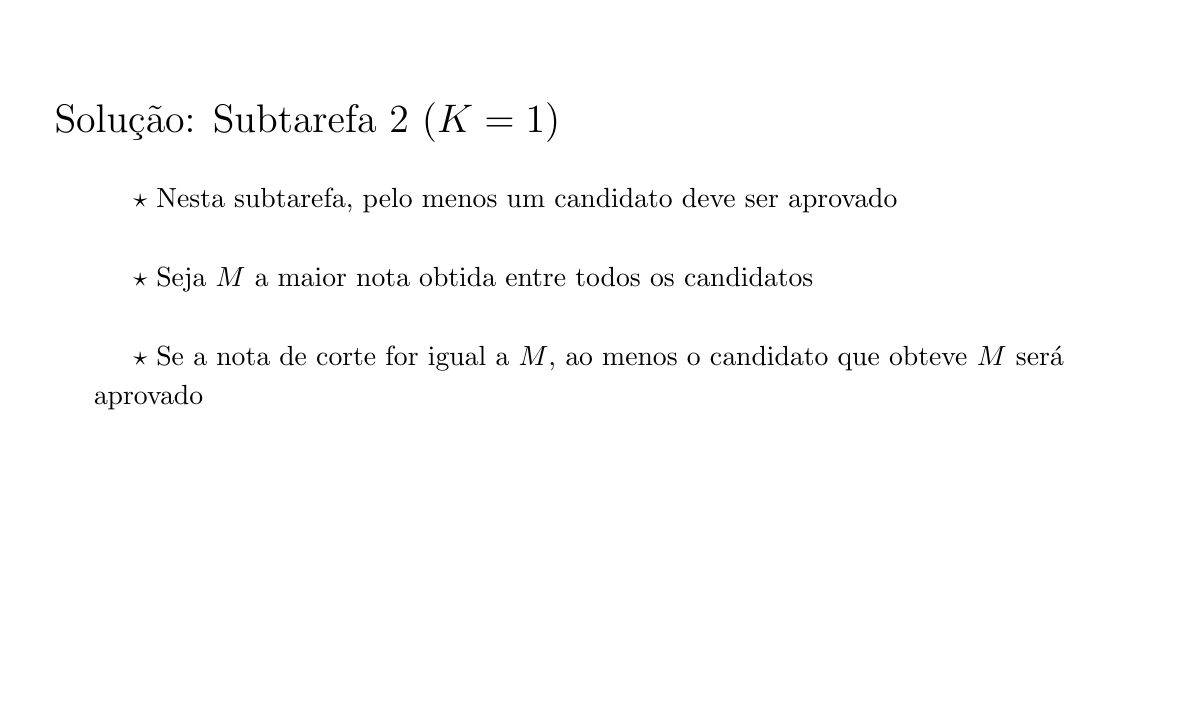
\begin{tikzpicture}
\node[draw,opacity=0] at (0, 0) {x};
\node[draw,opacity=0] at (14, 8) {x};

	\node[anchor=west] (title) at (0.0, 7.0) { \Large \bbbold{Solução: Subtarefa 2 ($K = 1$)} };


	\node[anchor=west] (a) at (1.0, 6.0) { $\star$ \bbtext{Nesta subtarefa, pelo menos um candidato deve ser aprovado} };


	\node[anchor=west] (b) at (1.0, 5.0) { $\star$ \bbtext{Seja $M$ a maior nota obtida entre todos os candidatos} };


	\node[anchor=west] (c) at (1.0, 4.0) { $\star$ \bbtext{Se a nota de corte for igual a $M$, ao menos o candidato que obteve $M$ será} };

	\node[anchor=west] (c1) at (0.5, 3.5) { \bbtext{aprovado} };

\end{tikzpicture}
\end{frame}
\begin{frame}[plain,t]
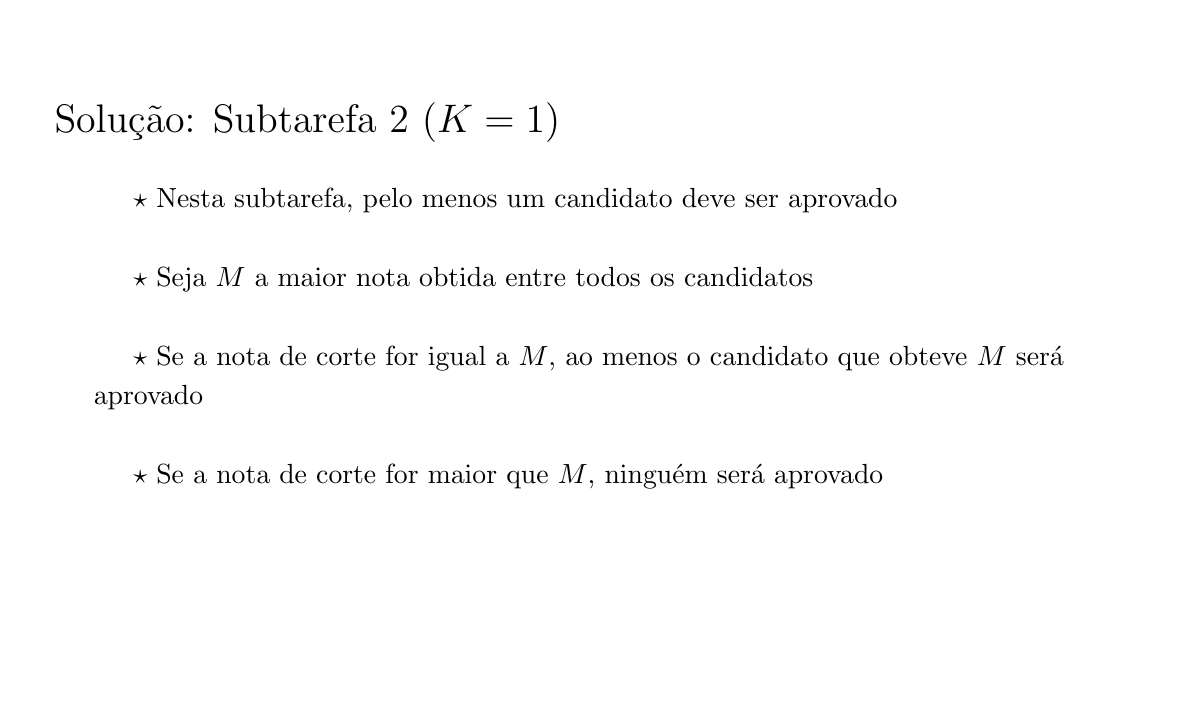
\begin{tikzpicture}
\node[draw,opacity=0] at (0, 0) {x};
\node[draw,opacity=0] at (14, 8) {x};

	\node[anchor=west] (title) at (0.0, 7.0) { \Large \bbbold{Solução: Subtarefa 2 ($K = 1$)} };


	\node[anchor=west] (a) at (1.0, 6.0) { $\star$ \bbtext{Nesta subtarefa, pelo menos um candidato deve ser aprovado} };


	\node[anchor=west] (b) at (1.0, 5.0) { $\star$ \bbtext{Seja $M$ a maior nota obtida entre todos os candidatos} };


	\node[anchor=west] (c) at (1.0, 4.0) { $\star$ \bbtext{Se a nota de corte for igual a $M$, ao menos o candidato que obteve $M$ será} };

	\node[anchor=west] (c1) at (0.5, 3.5) { \bbtext{aprovado} };


	\node[anchor=west] (d) at (1.0, 2.5) { $\star$ \bbtext{Se a nota de corte for maior que $M$, ninguém será aprovado} };

\end{tikzpicture}
\end{frame}
\begin{frame}[plain,t]
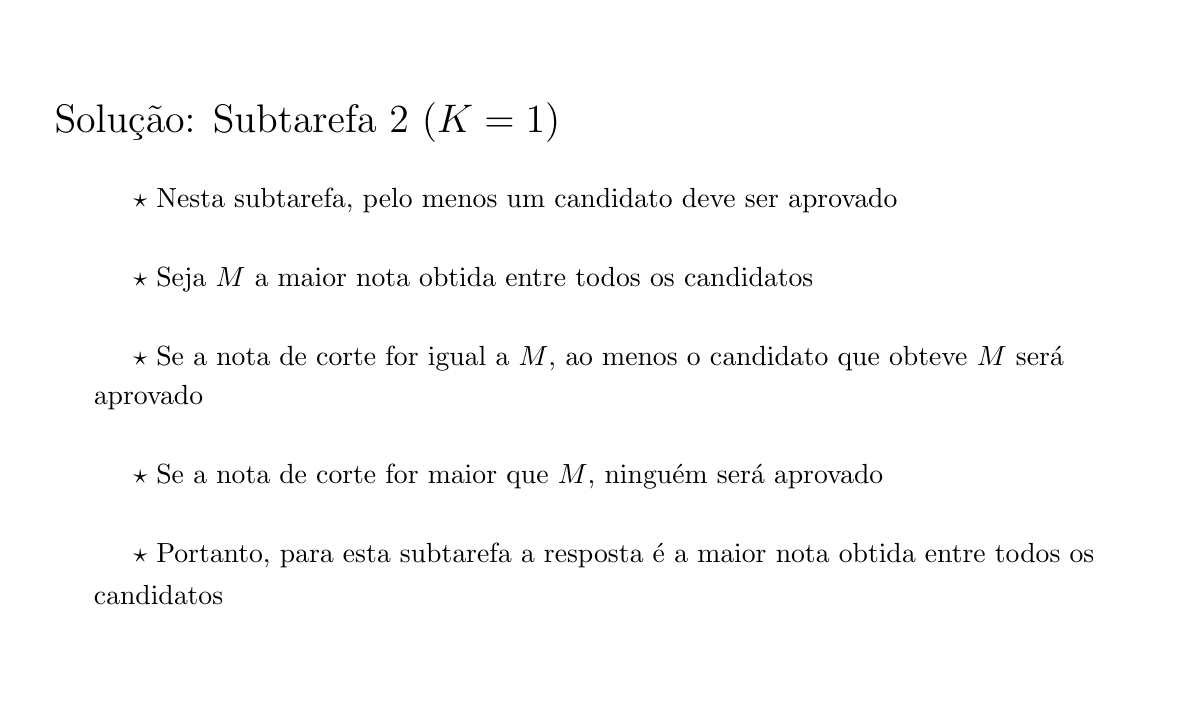
\begin{tikzpicture}
\node[draw,opacity=0] at (0, 0) {x};
\node[draw,opacity=0] at (14, 8) {x};

	\node[anchor=west] (title) at (0.0, 7.0) { \Large \bbbold{Solução: Subtarefa 2 ($K = 1$)} };


	\node[anchor=west] (a) at (1.0, 6.0) { $\star$ \bbtext{Nesta subtarefa, pelo menos um candidato deve ser aprovado} };


	\node[anchor=west] (b) at (1.0, 5.0) { $\star$ \bbtext{Seja $M$ a maior nota obtida entre todos os candidatos} };


	\node[anchor=west] (c) at (1.0, 4.0) { $\star$ \bbtext{Se a nota de corte for igual a $M$, ao menos o candidato que obteve $M$ será} };

	\node[anchor=west] (c1) at (0.5, 3.5) { \bbtext{aprovado} };


	\node[anchor=west] (d) at (1.0, 2.5) { $\star$ \bbtext{Se a nota de corte for maior que $M$, ninguém será aprovado} };


	\node[anchor=west] (e) at (1.0, 1.5) { $\star$ \bbtext{Portanto, para esta subtarefa a resposta é a maior nota obtida entre todos os} };

	\node[anchor=west] (e1) at (0.5, 1.0) { \bbtext{candidatos} };

\end{tikzpicture}
\end{frame}
\begin{frame}[plain,t]
\begin{tikzpicture}
\node[draw,opacity=0] at (0, 0) {x};
\node[draw,opacity=0] at (14, 8) {x};

	\node[anchor=west] (line1) at (1.0, 8.0) { \inputline{c}{1}{codes/sub2.c} };

	\node[anchor=west] (line2) at (1.0, 7.62) { \inputline{c}{2}{codes/sub2.c} };

	\node[anchor=west] (line3) at (1.0, 7.24) { \inputline{c}{3}{codes/sub2.c} };

	\node[anchor=west] (line4) at (1.0, 6.86) { \inputline{c}{4}{codes/sub2.c} };
















	\node[anchor=west] (line20) at (1.0, 0.76) { \inputline{c}{20}{codes/sub2.c} };

	\node[anchor=west] (line21) at (1.0, 0.38) { \inputline{c}{21}{codes/sub2.c} };

	\node[anchor=west] (line22) at (1.0, -0.0) { \inputline{c}{22}{codes/sub2.c} };


\end{tikzpicture}
\end{frame}
\begin{frame}[plain,t]
\begin{tikzpicture}
\node[draw,opacity=0] at (0, 0) {x};
\node[draw,opacity=0] at (14, 8) {x};

	\node[anchor=west] (line1) at (1.0, 8.0) { \inputline{c}{1}{codes/sub2.c} };

	\node[anchor=west] (line2) at (1.0, 7.62) { \inputline{c}{2}{codes/sub2.c} };

	\node[anchor=west] (line3) at (1.0, 7.24) { \inputline{c}{3}{codes/sub2.c} };

	\node[anchor=west] (line4) at (1.0, 6.86) { \inputline{c}{4}{codes/sub2.c} };

	\node[anchor=west] (line5) at (1.0, 6.48) { \inputline{c}{5}{codes/sub2.c} };

	\node[anchor=west] (line6) at (1.0, 6.1) { \inputline{c}{6}{codes/sub2.c} };














	\node[anchor=west] (line20) at (1.0, 0.76) { \inputline{c}{20}{codes/sub2.c} };

	\node[anchor=west] (line21) at (1.0, 0.38) { \inputline{c}{21}{codes/sub2.c} };

	\node[anchor=west] (line22) at (1.0, -0.0) { \inputline{c}{22}{codes/sub2.c} };




\end{tikzpicture}
\end{frame}
\begin{frame}[plain,t]
\begin{tikzpicture}
\node[draw,opacity=0] at (0, 0) {x};
\node[draw,opacity=0] at (14, 8) {x};

	\node[anchor=west] (line1) at (1.0, 8.0) { \inputline{c}{1}{codes/sub2.c} };

	\node[anchor=west] (line2) at (1.0, 7.62) { \inputline{c}{2}{codes/sub2.c} };

	\node[anchor=west] (line3) at (1.0, 7.24) { \inputline{c}{3}{codes/sub2.c} };

	\node[anchor=west] (line4) at (1.0, 6.86) { \inputline{c}{4}{codes/sub2.c} };

	\node[anchor=west] (line5) at (1.0, 6.48) { \inputline{c}{5}{codes/sub2.c} };

	\node[anchor=west] (line6) at (1.0, 6.1) { \inputline{c}{6}{codes/sub2.c} };


	\node[anchor=west] (line8) at (1.0, 5.33) { \inputline{c}{8}{codes/sub2.c} };












	\node[anchor=west] (line20) at (1.0, 0.76) { \inputline{c}{20}{codes/sub2.c} };

	\node[anchor=west] (line21) at (1.0, 0.38) { \inputline{c}{21}{codes/sub2.c} };

	\node[anchor=west] (line22) at (1.0, -0.0) { \inputline{c}{22}{codes/sub2.c} };






\end{tikzpicture}
\end{frame}
\begin{frame}[plain,t]
\begin{tikzpicture}
\node[draw,opacity=0] at (0, 0) {x};
\node[draw,opacity=0] at (14, 8) {x};

	\node[anchor=west] (line1) at (1.0, 8.0) { \inputline{c}{1}{codes/sub2.c} };

	\node[anchor=west] (line2) at (1.0, 7.62) { \inputline{c}{2}{codes/sub2.c} };

	\node[anchor=west] (line3) at (1.0, 7.24) { \inputline{c}{3}{codes/sub2.c} };

	\node[anchor=west] (line4) at (1.0, 6.86) { \inputline{c}{4}{codes/sub2.c} };

	\node[anchor=west] (line5) at (1.0, 6.48) { \inputline{c}{5}{codes/sub2.c} };

	\node[anchor=west] (line6) at (1.0, 6.1) { \inputline{c}{6}{codes/sub2.c} };


	\node[anchor=west] (line8) at (1.0, 5.33) { \inputline{c}{8}{codes/sub2.c} };


	\node[anchor=west] (line10) at (1.0, 4.57) { \inputline{c}{10}{codes/sub2.c} };

	\node[anchor=west] (line11) at (1.0, 4.19) { \inputline{c}{11}{codes/sub2.c} };






	\node[anchor=west] (line17) at (1.0, 1.9) { \inputline{c}{17}{codes/sub2.c} };



	\node[anchor=west] (line20) at (1.0, 0.76) { \inputline{c}{20}{codes/sub2.c} };

	\node[anchor=west] (line21) at (1.0, 0.38) { \inputline{c}{21}{codes/sub2.c} };

	\node[anchor=west] (line22) at (1.0, -0.0) { \inputline{c}{22}{codes/sub2.c} };








\end{tikzpicture}
\end{frame}
\begin{frame}[plain,t]
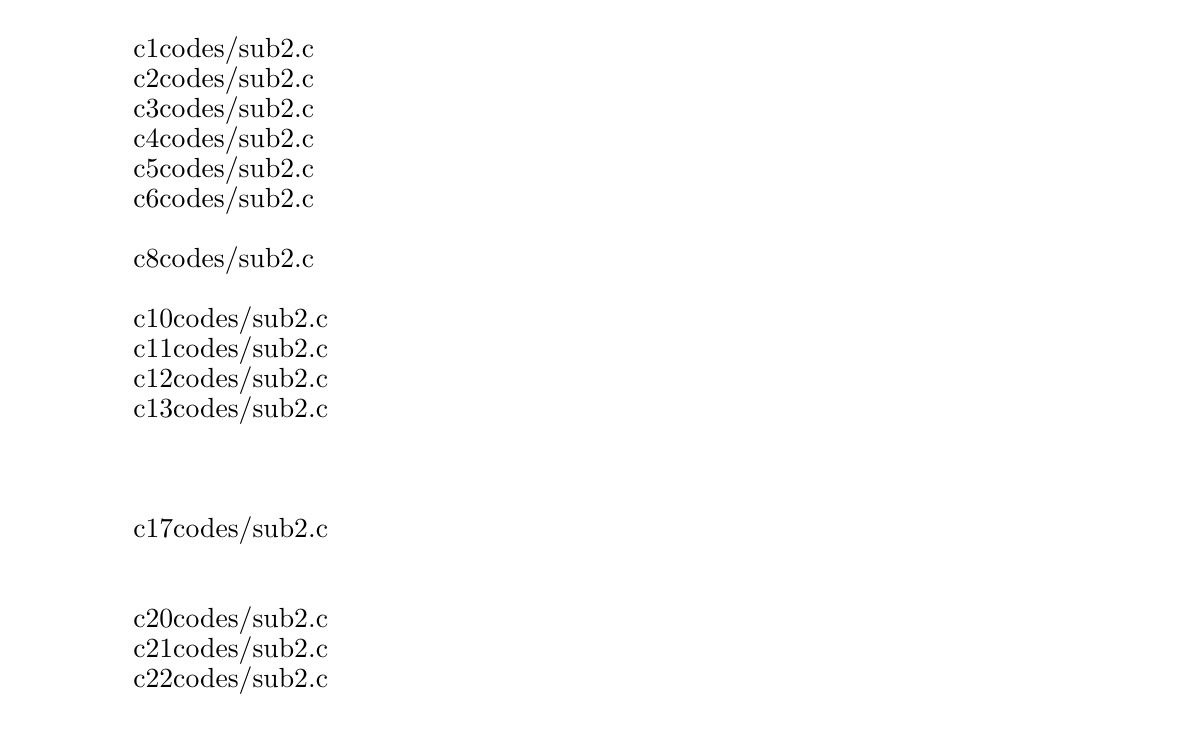
\begin{tikzpicture}
\node[draw,opacity=0] at (0, 0) {x};
\node[draw,opacity=0] at (14, 8) {x};

	\node[anchor=west] (line1) at (1.0, 8.0) { \inputline{c}{1}{codes/sub2.c} };

	\node[anchor=west] (line2) at (1.0, 7.62) { \inputline{c}{2}{codes/sub2.c} };

	\node[anchor=west] (line3) at (1.0, 7.24) { \inputline{c}{3}{codes/sub2.c} };

	\node[anchor=west] (line4) at (1.0, 6.86) { \inputline{c}{4}{codes/sub2.c} };

	\node[anchor=west] (line5) at (1.0, 6.48) { \inputline{c}{5}{codes/sub2.c} };

	\node[anchor=west] (line6) at (1.0, 6.1) { \inputline{c}{6}{codes/sub2.c} };


	\node[anchor=west] (line8) at (1.0, 5.33) { \inputline{c}{8}{codes/sub2.c} };


	\node[anchor=west] (line10) at (1.0, 4.57) { \inputline{c}{10}{codes/sub2.c} };

	\node[anchor=west] (line11) at (1.0, 4.19) { \inputline{c}{11}{codes/sub2.c} };

	\node[anchor=west] (line12) at (1.0, 3.81) { \inputline{c}{12}{codes/sub2.c} };

	\node[anchor=west] (line13) at (1.0, 3.43) { \inputline{c}{13}{codes/sub2.c} };




	\node[anchor=west] (line17) at (1.0, 1.9) { \inputline{c}{17}{codes/sub2.c} };



	\node[anchor=west] (line20) at (1.0, 0.76) { \inputline{c}{20}{codes/sub2.c} };

	\node[anchor=west] (line21) at (1.0, 0.38) { \inputline{c}{21}{codes/sub2.c} };

	\node[anchor=west] (line22) at (1.0, -0.0) { \inputline{c}{22}{codes/sub2.c} };









\end{tikzpicture}
\end{frame}
\begin{frame}[plain,t]
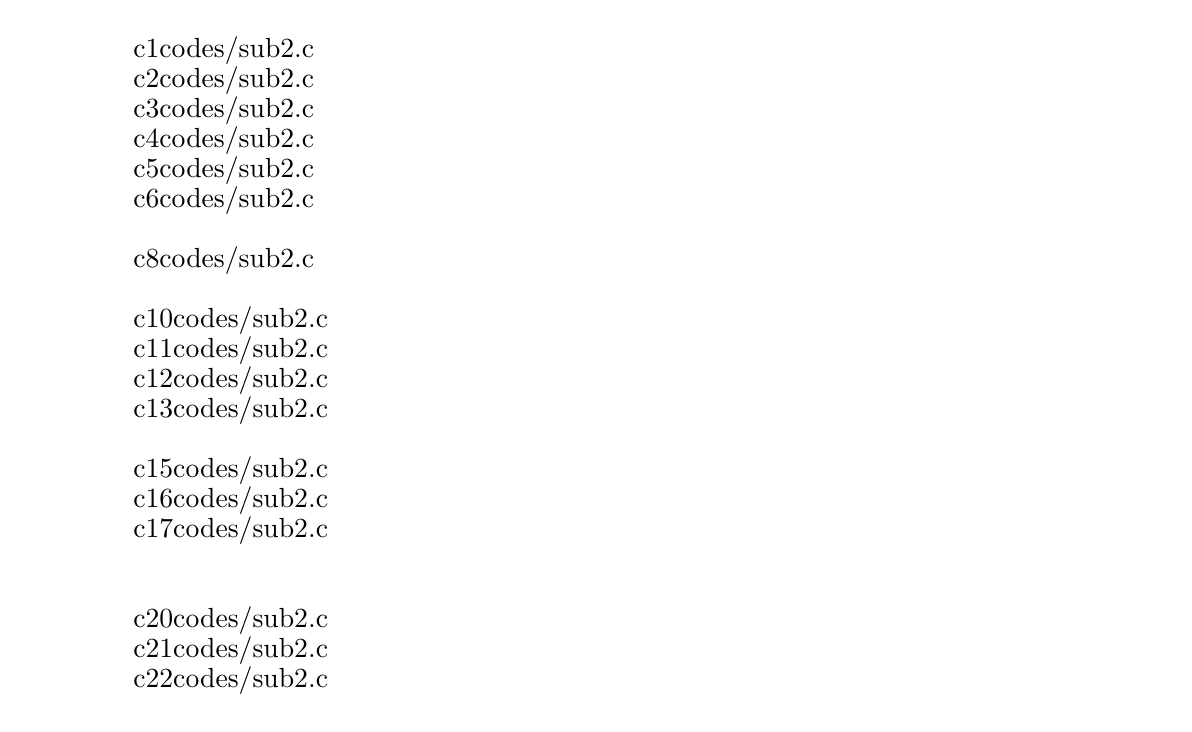
\begin{tikzpicture}
\node[draw,opacity=0] at (0, 0) {x};
\node[draw,opacity=0] at (14, 8) {x};

	\node[anchor=west] (line1) at (1.0, 8.0) { \inputline{c}{1}{codes/sub2.c} };

	\node[anchor=west] (line2) at (1.0, 7.62) { \inputline{c}{2}{codes/sub2.c} };

	\node[anchor=west] (line3) at (1.0, 7.24) { \inputline{c}{3}{codes/sub2.c} };

	\node[anchor=west] (line4) at (1.0, 6.86) { \inputline{c}{4}{codes/sub2.c} };

	\node[anchor=west] (line5) at (1.0, 6.48) { \inputline{c}{5}{codes/sub2.c} };

	\node[anchor=west] (line6) at (1.0, 6.1) { \inputline{c}{6}{codes/sub2.c} };


	\node[anchor=west] (line8) at (1.0, 5.33) { \inputline{c}{8}{codes/sub2.c} };


	\node[anchor=west] (line10) at (1.0, 4.57) { \inputline{c}{10}{codes/sub2.c} };

	\node[anchor=west] (line11) at (1.0, 4.19) { \inputline{c}{11}{codes/sub2.c} };

	\node[anchor=west] (line12) at (1.0, 3.81) { \inputline{c}{12}{codes/sub2.c} };

	\node[anchor=west] (line13) at (1.0, 3.43) { \inputline{c}{13}{codes/sub2.c} };


	\node[anchor=west] (line15) at (1.0, 2.67) { \inputline{c}{15}{codes/sub2.c} };

	\node[anchor=west] (line16) at (1.0, 2.29) { \inputline{c}{16}{codes/sub2.c} };

	\node[anchor=west] (line17) at (1.0, 1.9) { \inputline{c}{17}{codes/sub2.c} };



	\node[anchor=west] (line20) at (1.0, 0.76) { \inputline{c}{20}{codes/sub2.c} };

	\node[anchor=west] (line21) at (1.0, 0.38) { \inputline{c}{21}{codes/sub2.c} };

	\node[anchor=west] (line22) at (1.0, -0.0) { \inputline{c}{22}{codes/sub2.c} };










\end{tikzpicture}
\end{frame}
\begin{frame}[plain,t]
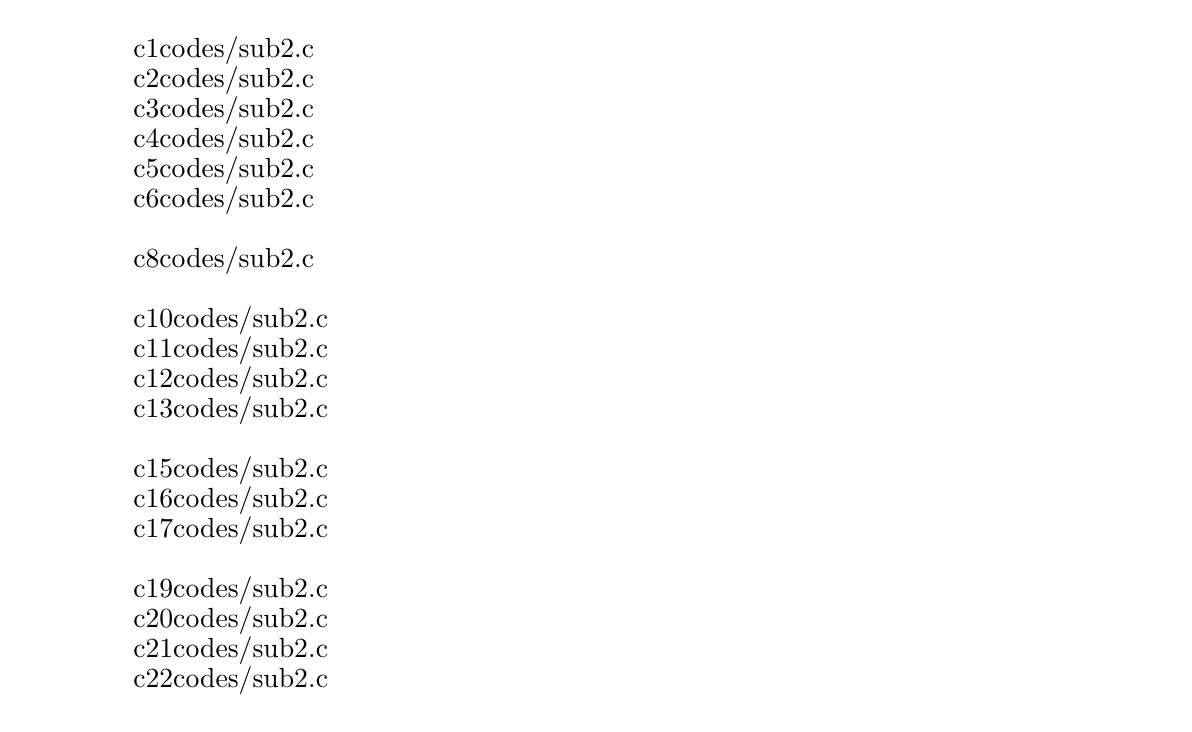
\begin{tikzpicture}
\node[draw,opacity=0] at (0, 0) {x};
\node[draw,opacity=0] at (14, 8) {x};

	\node[anchor=west] (line1) at (1.0, 8.0) { \inputline{c}{1}{codes/sub2.c} };

	\node[anchor=west] (line2) at (1.0, 7.62) { \inputline{c}{2}{codes/sub2.c} };

	\node[anchor=west] (line3) at (1.0, 7.24) { \inputline{c}{3}{codes/sub2.c} };

	\node[anchor=west] (line4) at (1.0, 6.86) { \inputline{c}{4}{codes/sub2.c} };

	\node[anchor=west] (line5) at (1.0, 6.48) { \inputline{c}{5}{codes/sub2.c} };

	\node[anchor=west] (line6) at (1.0, 6.1) { \inputline{c}{6}{codes/sub2.c} };


	\node[anchor=west] (line8) at (1.0, 5.33) { \inputline{c}{8}{codes/sub2.c} };


	\node[anchor=west] (line10) at (1.0, 4.57) { \inputline{c}{10}{codes/sub2.c} };

	\node[anchor=west] (line11) at (1.0, 4.19) { \inputline{c}{11}{codes/sub2.c} };

	\node[anchor=west] (line12) at (1.0, 3.81) { \inputline{c}{12}{codes/sub2.c} };

	\node[anchor=west] (line13) at (1.0, 3.43) { \inputline{c}{13}{codes/sub2.c} };


	\node[anchor=west] (line15) at (1.0, 2.67) { \inputline{c}{15}{codes/sub2.c} };

	\node[anchor=west] (line16) at (1.0, 2.29) { \inputline{c}{16}{codes/sub2.c} };

	\node[anchor=west] (line17) at (1.0, 1.9) { \inputline{c}{17}{codes/sub2.c} };


	\node[anchor=west] (line19) at (1.0, 1.14) { \inputline{c}{19}{codes/sub2.c} };

	\node[anchor=west] (line20) at (1.0, 0.76) { \inputline{c}{20}{codes/sub2.c} };

	\node[anchor=west] (line21) at (1.0, 0.38) { \inputline{c}{21}{codes/sub2.c} };

	\node[anchor=west] (line22) at (1.0, -0.0) { \inputline{c}{22}{codes/sub2.c} };











\end{tikzpicture}
\end{frame}
\begin{frame}[plain,t]
\begin{tikzpicture}
\node[draw,opacity=0] at (0, 0) {x};
\node[draw,opacity=0] at (14, 8) {x};

	\node[anchor=west] (title) at (0.0, 7.0) { \Large \bbbold{Solução: Subtarefa 4 ($A_i \leq 2$)} };

\end{tikzpicture}
\end{frame}
\begin{frame}[plain,t]
\begin{tikzpicture}
\node[draw,opacity=0] at (0, 0) {x};
\node[draw,opacity=0] at (14, 8) {x};

	\node[anchor=west] (title) at (0.0, 7.0) { \Large \bbbold{Solução: Subtarefa 4 ($A_i \leq 2$)} };


	\node[anchor=west] (a) at (1.0, 6.0) { $\star$ \bbtext{Nesta subtarefa, todos candidatos tiraram ou nota 1 ou nota 2} };
\end{tikzpicture}
\end{frame}
\begin{frame}[plain,t]
\begin{tikzpicture}
\node[draw,opacity=0] at (0, 0) {x};
\node[draw,opacity=0] at (14, 8) {x};

	\node[anchor=west] (title) at (0.0, 7.0) { \Large \bbbold{Solução: Subtarefa 4 ($A_i \leq 2$)} };


	\node[anchor=west] (a) at (1.0, 6.0) { $\star$ \bbtext{Nesta subtarefa, todos candidatos tiraram ou nota 1 ou nota 2} };

	\node[anchor=west] (b) at (1.0, 5.0) { $\star$ \bbtext{Só há duas alternativas para a nota de corte: $C = 1$ e $C = 2$} };

\end{tikzpicture}
\end{frame}
\begin{frame}[plain,t]
\begin{tikzpicture}
\node[draw,opacity=0] at (0, 0) {x};
\node[draw,opacity=0] at (14, 8) {x};

	\node[anchor=west] (title) at (0.0, 7.0) { \Large \bbbold{Solução: Subtarefa 4 ($A_i \leq 2$)} };


	\node[anchor=west] (a) at (1.0, 6.0) { $\star$ \bbtext{Nesta subtarefa, todos candidatos tiraram ou nota 1 ou nota 2} };

	\node[anchor=west] (b) at (1.0, 5.0) { $\star$ \bbtext{Só há duas alternativas para a nota de corte: $C = 1$ e $C = 2$} };


	\node[anchor=west] (c) at (1.0, 4.0) { $\star$ \bbtext{Se a nota de corte for igual a $1$, todos serão aprovados} };

\end{tikzpicture}
\end{frame}
\begin{frame}[plain,t]
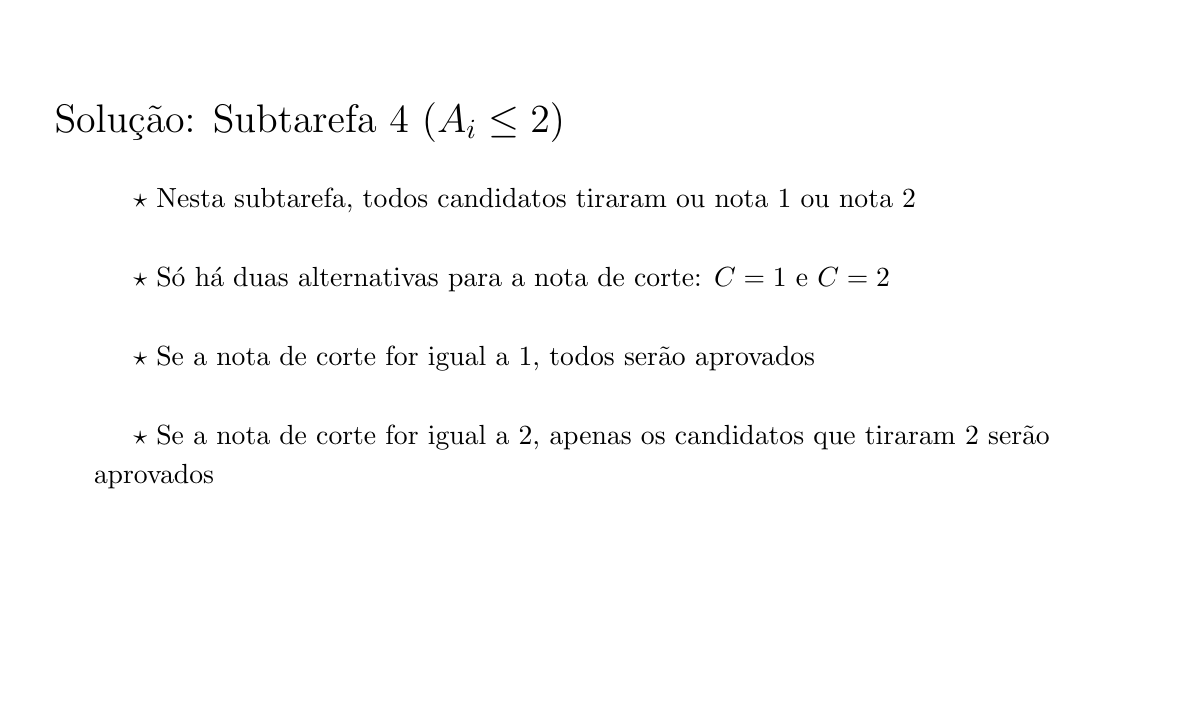
\begin{tikzpicture}
\node[draw,opacity=0] at (0, 0) {x};
\node[draw,opacity=0] at (14, 8) {x};

	\node[anchor=west] (title) at (0.0, 7.0) { \Large \bbbold{Solução: Subtarefa 4 ($A_i \leq 2$)} };


	\node[anchor=west] (a) at (1.0, 6.0) { $\star$ \bbtext{Nesta subtarefa, todos candidatos tiraram ou nota 1 ou nota 2} };

	\node[anchor=west] (b) at (1.0, 5.0) { $\star$ \bbtext{Só há duas alternativas para a nota de corte: $C = 1$ e $C = 2$} };


	\node[anchor=west] (c) at (1.0, 4.0) { $\star$ \bbtext{Se a nota de corte for igual a $1$, todos serão aprovados} };


	\node[anchor=west] (d) at (1.0, 3.0) { $\star$ \bbtext{Se a nota de corte for igual a $2$, apenas os candidatos que tiraram 2 serão} };

	\node[anchor=west] (d1) at (0.5, 2.5) { \bbtext{aprovados} };


\end{tikzpicture}
\end{frame}
\begin{frame}[plain,t]
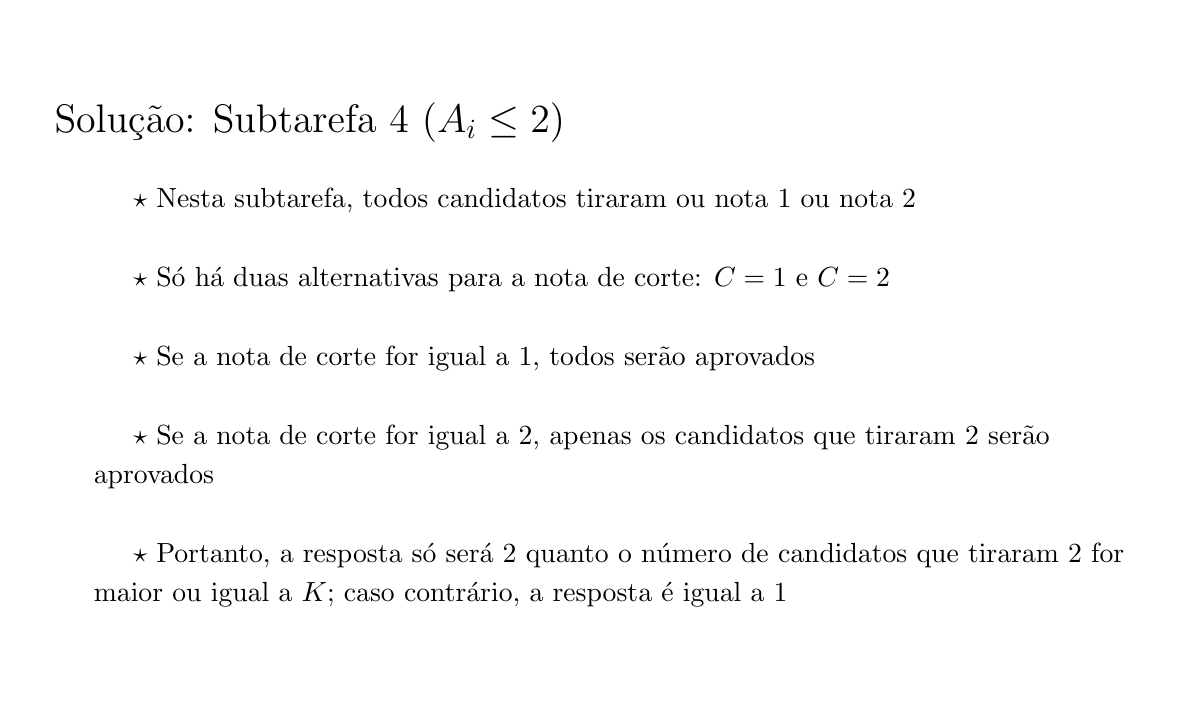
\begin{tikzpicture}
\node[draw,opacity=0] at (0, 0) {x};
\node[draw,opacity=0] at (14, 8) {x};

	\node[anchor=west] (title) at (0.0, 7.0) { \Large \bbbold{Solução: Subtarefa 4 ($A_i \leq 2$)} };


	\node[anchor=west] (a) at (1.0, 6.0) { $\star$ \bbtext{Nesta subtarefa, todos candidatos tiraram ou nota 1 ou nota 2} };

	\node[anchor=west] (b) at (1.0, 5.0) { $\star$ \bbtext{Só há duas alternativas para a nota de corte: $C = 1$ e $C = 2$} };


	\node[anchor=west] (c) at (1.0, 4.0) { $\star$ \bbtext{Se a nota de corte for igual a $1$, todos serão aprovados} };


	\node[anchor=west] (d) at (1.0, 3.0) { $\star$ \bbtext{Se a nota de corte for igual a $2$, apenas os candidatos que tiraram 2 serão} };

	\node[anchor=west] (d1) at (0.5, 2.5) { \bbtext{aprovados} };



	\node[anchor=west] (e) at (1.0, 1.5) { $\star$ \bbtext{Portanto, a resposta só será $2$ quanto o número de candidatos que tiraram 2 for} };

	\node[anchor=west] (e1) at (0.5, 1.0) { \bbtext{maior ou igual a $K$; caso contrário, a resposta é igual a 1} };

\end{tikzpicture}
\end{frame}
\begin{frame}[plain,t]
\begin{tikzpicture}
\node[draw,opacity=0] at (0, 0) {x};
\node[draw,opacity=0] at (14, 8) {x};

	\node[anchor=west] (line1) at (1.0, 8.0) { \inputline{c}{1}{codes/sub4.c} };

	\node[anchor=west] (line2) at (1.0, 7.62) { \inputline{c}{2}{codes/sub4.c} };

	\node[anchor=west] (line3) at (1.0, 7.24) { \inputline{c}{3}{codes/sub4.c} };

	\node[anchor=west] (line4) at (1.0, 6.86) { \inputline{c}{4}{codes/sub4.c} };
















	\node[anchor=west] (line20) at (1.0, 0.76) { \inputline{c}{20}{codes/sub4.c} };

	\node[anchor=west] (line21) at (1.0, 0.38) { \inputline{c}{21}{codes/sub4.c} };

	\node[anchor=west] (line22) at (1.0, -0.0) { \inputline{c}{22}{codes/sub4.c} };


\end{tikzpicture}
\end{frame}
\begin{frame}[plain,t]
\begin{tikzpicture}
\node[draw,opacity=0] at (0, 0) {x};
\node[draw,opacity=0] at (14, 8) {x};

	\node[anchor=west] (line1) at (1.0, 8.0) { \inputline{c}{1}{codes/sub4.c} };

	\node[anchor=west] (line2) at (1.0, 7.62) { \inputline{c}{2}{codes/sub4.c} };

	\node[anchor=west] (line3) at (1.0, 7.24) { \inputline{c}{3}{codes/sub4.c} };

	\node[anchor=west] (line4) at (1.0, 6.86) { \inputline{c}{4}{codes/sub4.c} };

	\node[anchor=west] (line5) at (1.0, 6.48) { \inputline{c}{5}{codes/sub4.c} };

	\node[anchor=west] (line6) at (1.0, 6.1) { \inputline{c}{6}{codes/sub4.c} };














	\node[anchor=west] (line20) at (1.0, 0.76) { \inputline{c}{20}{codes/sub4.c} };

	\node[anchor=west] (line21) at (1.0, 0.38) { \inputline{c}{21}{codes/sub4.c} };

	\node[anchor=west] (line22) at (1.0, -0.0) { \inputline{c}{22}{codes/sub4.c} };




\end{tikzpicture}
\end{frame}
\begin{frame}[plain,t]
\begin{tikzpicture}
\node[draw,opacity=0] at (0, 0) {x};
\node[draw,opacity=0] at (14, 8) {x};

	\node[anchor=west] (line1) at (1.0, 8.0) { \inputline{c}{1}{codes/sub4.c} };

	\node[anchor=west] (line2) at (1.0, 7.62) { \inputline{c}{2}{codes/sub4.c} };

	\node[anchor=west] (line3) at (1.0, 7.24) { \inputline{c}{3}{codes/sub4.c} };

	\node[anchor=west] (line4) at (1.0, 6.86) { \inputline{c}{4}{codes/sub4.c} };

	\node[anchor=west] (line5) at (1.0, 6.48) { \inputline{c}{5}{codes/sub4.c} };

	\node[anchor=west] (line6) at (1.0, 6.1) { \inputline{c}{6}{codes/sub4.c} };


	\node[anchor=west] (line8) at (1.0, 5.33) { \inputline{c}{8}{codes/sub4.c} };












	\node[anchor=west] (line20) at (1.0, 0.76) { \inputline{c}{20}{codes/sub4.c} };

	\node[anchor=west] (line21) at (1.0, 0.38) { \inputline{c}{21}{codes/sub4.c} };

	\node[anchor=west] (line22) at (1.0, -0.0) { \inputline{c}{22}{codes/sub4.c} };






\end{tikzpicture}
\end{frame}
\begin{frame}[plain,t]
\begin{tikzpicture}
\node[draw,opacity=0] at (0, 0) {x};
\node[draw,opacity=0] at (14, 8) {x};

	\node[anchor=west] (line1) at (1.0, 8.0) { \inputline{c}{1}{codes/sub4.c} };

	\node[anchor=west] (line2) at (1.0, 7.62) { \inputline{c}{2}{codes/sub4.c} };

	\node[anchor=west] (line3) at (1.0, 7.24) { \inputline{c}{3}{codes/sub4.c} };

	\node[anchor=west] (line4) at (1.0, 6.86) { \inputline{c}{4}{codes/sub4.c} };

	\node[anchor=west] (line5) at (1.0, 6.48) { \inputline{c}{5}{codes/sub4.c} };

	\node[anchor=west] (line6) at (1.0, 6.1) { \inputline{c}{6}{codes/sub4.c} };


	\node[anchor=west] (line8) at (1.0, 5.33) { \inputline{c}{8}{codes/sub4.c} };


	\node[anchor=west] (line10) at (1.0, 4.57) { \inputline{c}{10}{codes/sub4.c} };

	\node[anchor=west] (line11) at (1.0, 4.19) { \inputline{c}{11}{codes/sub4.c} };






	\node[anchor=west] (line17) at (1.0, 1.9) { \inputline{c}{17}{codes/sub4.c} };



	\node[anchor=west] (line20) at (1.0, 0.76) { \inputline{c}{20}{codes/sub4.c} };

	\node[anchor=west] (line21) at (1.0, 0.38) { \inputline{c}{21}{codes/sub4.c} };

	\node[anchor=west] (line22) at (1.0, -0.0) { \inputline{c}{22}{codes/sub4.c} };








\end{tikzpicture}
\end{frame}
\begin{frame}[plain,t]
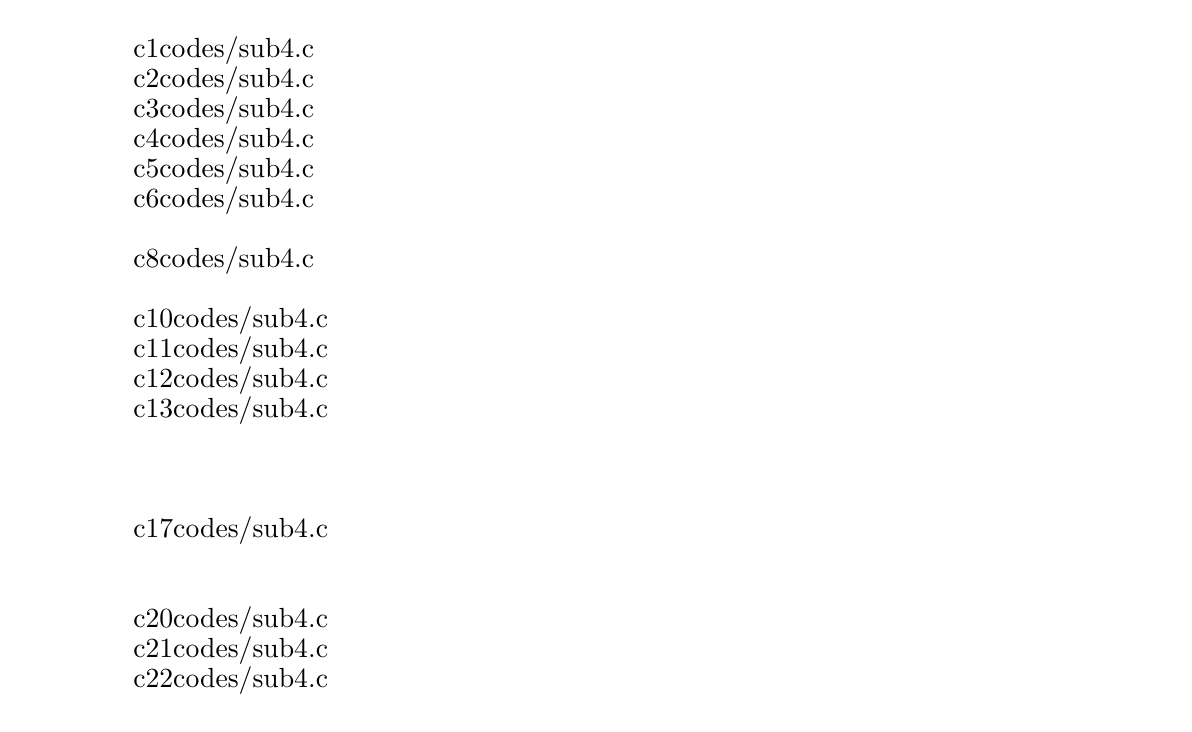
\begin{tikzpicture}
\node[draw,opacity=0] at (0, 0) {x};
\node[draw,opacity=0] at (14, 8) {x};

	\node[anchor=west] (line1) at (1.0, 8.0) { \inputline{c}{1}{codes/sub4.c} };

	\node[anchor=west] (line2) at (1.0, 7.62) { \inputline{c}{2}{codes/sub4.c} };

	\node[anchor=west] (line3) at (1.0, 7.24) { \inputline{c}{3}{codes/sub4.c} };

	\node[anchor=west] (line4) at (1.0, 6.86) { \inputline{c}{4}{codes/sub4.c} };

	\node[anchor=west] (line5) at (1.0, 6.48) { \inputline{c}{5}{codes/sub4.c} };

	\node[anchor=west] (line6) at (1.0, 6.1) { \inputline{c}{6}{codes/sub4.c} };


	\node[anchor=west] (line8) at (1.0, 5.33) { \inputline{c}{8}{codes/sub4.c} };


	\node[anchor=west] (line10) at (1.0, 4.57) { \inputline{c}{10}{codes/sub4.c} };

	\node[anchor=west] (line11) at (1.0, 4.19) { \inputline{c}{11}{codes/sub4.c} };

	\node[anchor=west] (line12) at (1.0, 3.81) { \inputline{c}{12}{codes/sub4.c} };

	\node[anchor=west] (line13) at (1.0, 3.43) { \inputline{c}{13}{codes/sub4.c} };




	\node[anchor=west] (line17) at (1.0, 1.9) { \inputline{c}{17}{codes/sub4.c} };



	\node[anchor=west] (line20) at (1.0, 0.76) { \inputline{c}{20}{codes/sub4.c} };

	\node[anchor=west] (line21) at (1.0, 0.38) { \inputline{c}{21}{codes/sub4.c} };

	\node[anchor=west] (line22) at (1.0, -0.0) { \inputline{c}{22}{codes/sub4.c} };









\end{tikzpicture}
\end{frame}
\begin{frame}[plain,t]
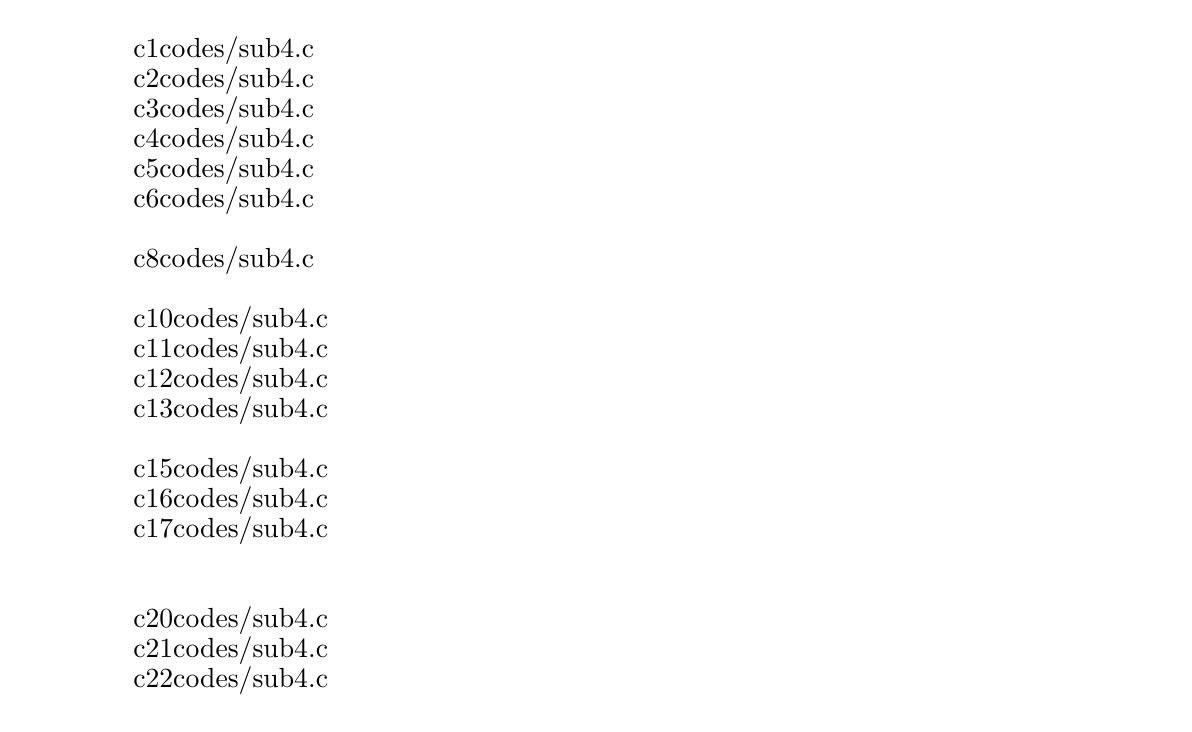
\begin{tikzpicture}
\node[draw,opacity=0] at (0, 0) {x};
\node[draw,opacity=0] at (14, 8) {x};

	\node[anchor=west] (line1) at (1.0, 8.0) { \inputline{c}{1}{codes/sub4.c} };

	\node[anchor=west] (line2) at (1.0, 7.62) { \inputline{c}{2}{codes/sub4.c} };

	\node[anchor=west] (line3) at (1.0, 7.24) { \inputline{c}{3}{codes/sub4.c} };

	\node[anchor=west] (line4) at (1.0, 6.86) { \inputline{c}{4}{codes/sub4.c} };

	\node[anchor=west] (line5) at (1.0, 6.48) { \inputline{c}{5}{codes/sub4.c} };

	\node[anchor=west] (line6) at (1.0, 6.1) { \inputline{c}{6}{codes/sub4.c} };


	\node[anchor=west] (line8) at (1.0, 5.33) { \inputline{c}{8}{codes/sub4.c} };


	\node[anchor=west] (line10) at (1.0, 4.57) { \inputline{c}{10}{codes/sub4.c} };

	\node[anchor=west] (line11) at (1.0, 4.19) { \inputline{c}{11}{codes/sub4.c} };

	\node[anchor=west] (line12) at (1.0, 3.81) { \inputline{c}{12}{codes/sub4.c} };

	\node[anchor=west] (line13) at (1.0, 3.43) { \inputline{c}{13}{codes/sub4.c} };


	\node[anchor=west] (line15) at (1.0, 2.67) { \inputline{c}{15}{codes/sub4.c} };

	\node[anchor=west] (line16) at (1.0, 2.29) { \inputline{c}{16}{codes/sub4.c} };

	\node[anchor=west] (line17) at (1.0, 1.9) { \inputline{c}{17}{codes/sub4.c} };



	\node[anchor=west] (line20) at (1.0, 0.76) { \inputline{c}{20}{codes/sub4.c} };

	\node[anchor=west] (line21) at (1.0, 0.38) { \inputline{c}{21}{codes/sub4.c} };

	\node[anchor=west] (line22) at (1.0, -0.0) { \inputline{c}{22}{codes/sub4.c} };










\end{tikzpicture}
\end{frame}
\begin{frame}[plain,t]
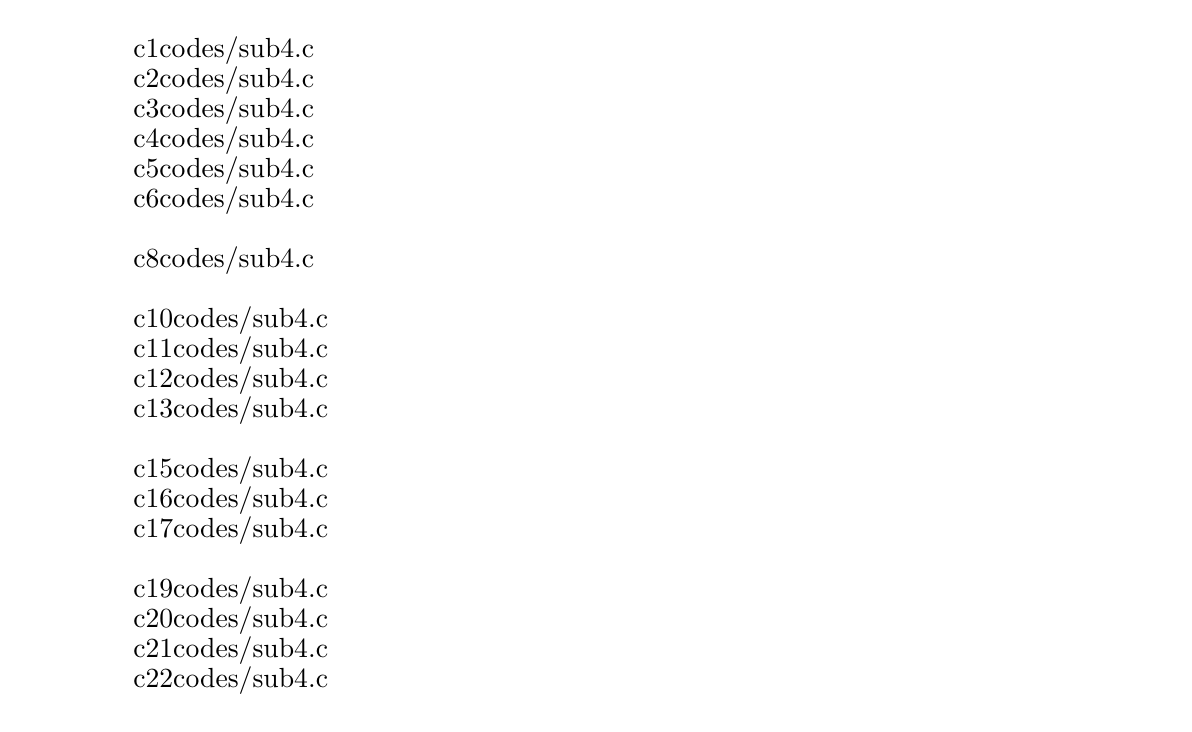
\begin{tikzpicture}
\node[draw,opacity=0] at (0, 0) {x};
\node[draw,opacity=0] at (14, 8) {x};

	\node[anchor=west] (line1) at (1.0, 8.0) { \inputline{c}{1}{codes/sub4.c} };

	\node[anchor=west] (line2) at (1.0, 7.62) { \inputline{c}{2}{codes/sub4.c} };

	\node[anchor=west] (line3) at (1.0, 7.24) { \inputline{c}{3}{codes/sub4.c} };

	\node[anchor=west] (line4) at (1.0, 6.86) { \inputline{c}{4}{codes/sub4.c} };

	\node[anchor=west] (line5) at (1.0, 6.48) { \inputline{c}{5}{codes/sub4.c} };

	\node[anchor=west] (line6) at (1.0, 6.1) { \inputline{c}{6}{codes/sub4.c} };


	\node[anchor=west] (line8) at (1.0, 5.33) { \inputline{c}{8}{codes/sub4.c} };


	\node[anchor=west] (line10) at (1.0, 4.57) { \inputline{c}{10}{codes/sub4.c} };

	\node[anchor=west] (line11) at (1.0, 4.19) { \inputline{c}{11}{codes/sub4.c} };

	\node[anchor=west] (line12) at (1.0, 3.81) { \inputline{c}{12}{codes/sub4.c} };

	\node[anchor=west] (line13) at (1.0, 3.43) { \inputline{c}{13}{codes/sub4.c} };


	\node[anchor=west] (line15) at (1.0, 2.67) { \inputline{c}{15}{codes/sub4.c} };

	\node[anchor=west] (line16) at (1.0, 2.29) { \inputline{c}{16}{codes/sub4.c} };

	\node[anchor=west] (line17) at (1.0, 1.9) { \inputline{c}{17}{codes/sub4.c} };


	\node[anchor=west] (line19) at (1.0, 1.14) { \inputline{c}{19}{codes/sub4.c} };

	\node[anchor=west] (line20) at (1.0, 0.76) { \inputline{c}{20}{codes/sub4.c} };

	\node[anchor=west] (line21) at (1.0, 0.38) { \inputline{c}{21}{codes/sub4.c} };

	\node[anchor=west] (line22) at (1.0, -0.0) { \inputline{c}{22}{codes/sub4.c} };











\end{tikzpicture}
\end{frame}
\begin{frame}[plain,t]
\begin{tikzpicture}
\node[draw,opacity=0] at (0, 0) {x};
\node[draw,opacity=0] at (14, 8) {x};

	\node[anchor=west] (title) at (0.0, 7.0) { \Large \bbbold{Solução: Subtarefa 3 ($K = 3$)} };

\end{tikzpicture}
\end{frame}
\begin{frame}[plain,t]
\begin{tikzpicture}
\node[draw,opacity=0] at (0, 0) {x};
\node[draw,opacity=0] at (14, 8) {x};

	\node[anchor=west] (title) at (0.0, 7.0) { \Large \bbbold{Solução: Subtarefa 3 ($K = 3$)} };


	\node[anchor=west] (a) at (1.0, 6.0) { $\star$ \bbtext{Nesta subtarefa deve ser classificados, no mínimo, 3 candidatos} };
\end{tikzpicture}
\end{frame}
\begin{frame}[plain,t]
\begin{tikzpicture}
\node[draw,opacity=0] at (0, 0) {x};
\node[draw,opacity=0] at (14, 8) {x};

	\node[anchor=west] (title) at (0.0, 7.0) { \Large \bbbold{Solução: Subtarefa 3 ($K = 3$)} };


	\node[anchor=west] (a) at (1.0, 6.0) { $\star$ \bbtext{Nesta subtarefa deve ser classificados, no mínimo, 3 candidatos} };

	\node[anchor=west] (b) at (1.0, 5.0) { $\star$ \bbtext{Na Subtarefa 1 a resposta era a nota do primeiro classificado} };

\end{tikzpicture}
\end{frame}
\begin{frame}[plain,t]
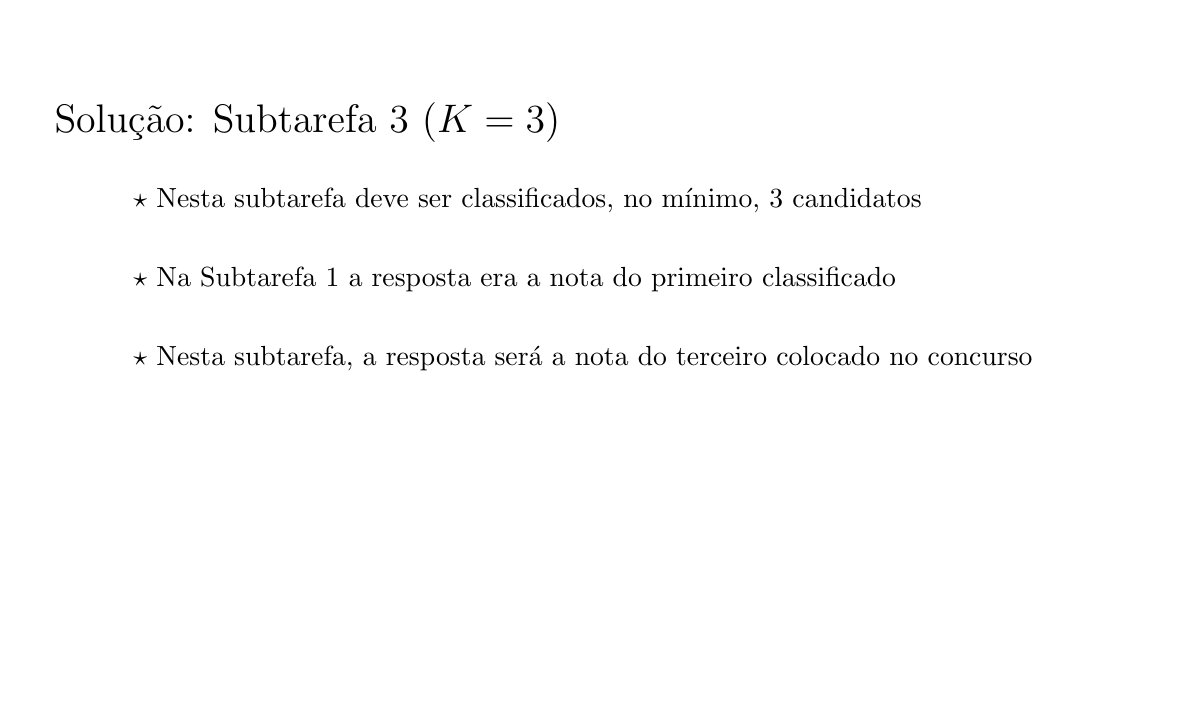
\begin{tikzpicture}
\node[draw,opacity=0] at (0, 0) {x};
\node[draw,opacity=0] at (14, 8) {x};

	\node[anchor=west] (title) at (0.0, 7.0) { \Large \bbbold{Solução: Subtarefa 3 ($K = 3$)} };


	\node[anchor=west] (a) at (1.0, 6.0) { $\star$ \bbtext{Nesta subtarefa deve ser classificados, no mínimo, 3 candidatos} };

	\node[anchor=west] (b) at (1.0, 5.0) { $\star$ \bbtext{Na Subtarefa 1 a resposta era a nota do primeiro classificado} };


	\node[anchor=west] (c) at (1.0, 4.0) { $\star$ \bbtext{Nesta subtarefa, a resposta será a nota do terceiro colocado no concurso} };

\end{tikzpicture}
\end{frame}
\begin{frame}[plain,t]
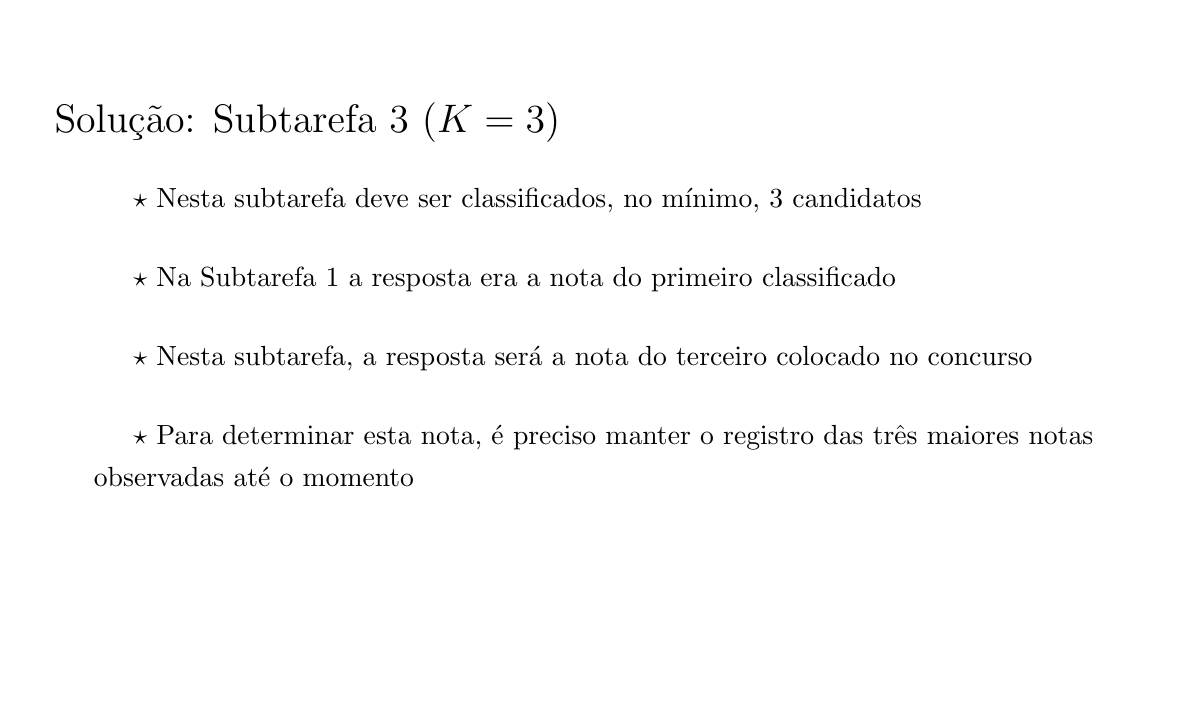
\begin{tikzpicture}
\node[draw,opacity=0] at (0, 0) {x};
\node[draw,opacity=0] at (14, 8) {x};

	\node[anchor=west] (title) at (0.0, 7.0) { \Large \bbbold{Solução: Subtarefa 3 ($K = 3$)} };


	\node[anchor=west] (a) at (1.0, 6.0) { $\star$ \bbtext{Nesta subtarefa deve ser classificados, no mínimo, 3 candidatos} };

	\node[anchor=west] (b) at (1.0, 5.0) { $\star$ \bbtext{Na Subtarefa 1 a resposta era a nota do primeiro classificado} };


	\node[anchor=west] (c) at (1.0, 4.0) { $\star$ \bbtext{Nesta subtarefa, a resposta será a nota do terceiro colocado no concurso} };


	\node[anchor=west] (d) at (1.0, 3.0) { $\star$ \bbtext{Para determinar esta nota, é preciso manter o registro das três maiores notas } };

	\node[anchor=west] (d1) at (0.5, 2.5) { \bbtext{observadas até o momento} };


\end{tikzpicture}
\end{frame}
\begin{frame}[plain,t]
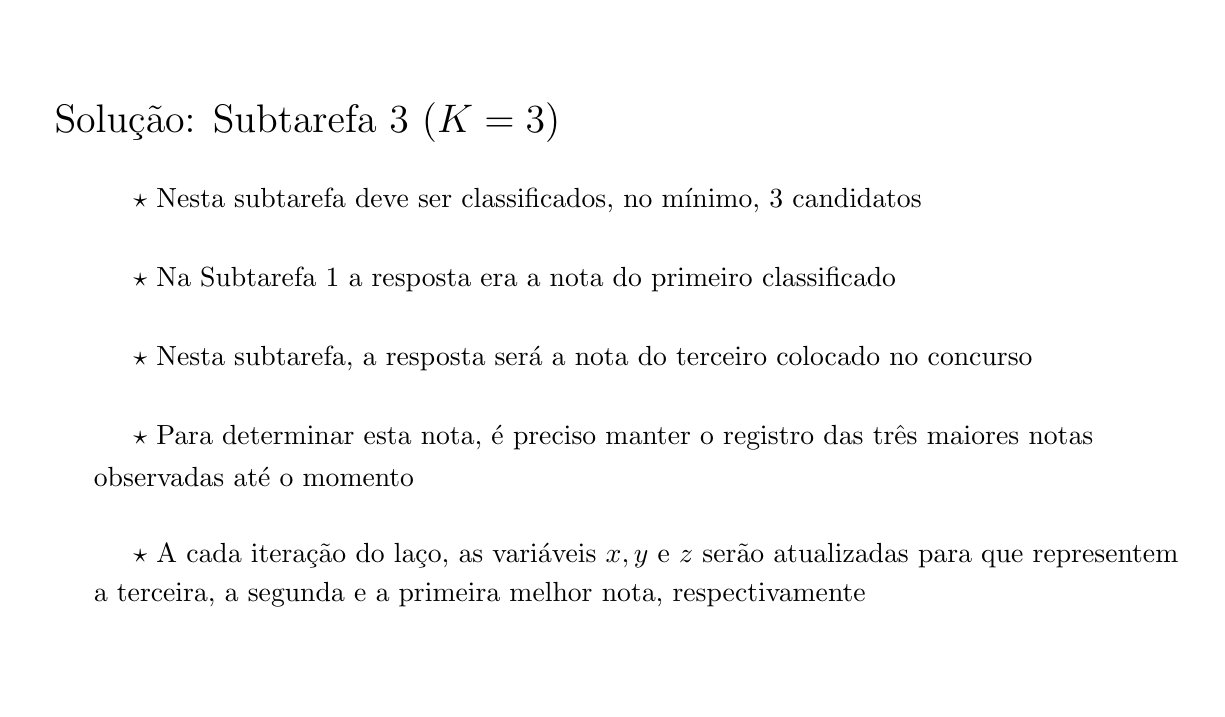
\begin{tikzpicture}
\node[draw,opacity=0] at (0, 0) {x};
\node[draw,opacity=0] at (14, 8) {x};

	\node[anchor=west] (title) at (0.0, 7.0) { \Large \bbbold{Solução: Subtarefa 3 ($K = 3$)} };


	\node[anchor=west] (a) at (1.0, 6.0) { $\star$ \bbtext{Nesta subtarefa deve ser classificados, no mínimo, 3 candidatos} };

	\node[anchor=west] (b) at (1.0, 5.0) { $\star$ \bbtext{Na Subtarefa 1 a resposta era a nota do primeiro classificado} };


	\node[anchor=west] (c) at (1.0, 4.0) { $\star$ \bbtext{Nesta subtarefa, a resposta será a nota do terceiro colocado no concurso} };


	\node[anchor=west] (d) at (1.0, 3.0) { $\star$ \bbtext{Para determinar esta nota, é preciso manter o registro das três maiores notas } };

	\node[anchor=west] (d1) at (0.5, 2.5) { \bbtext{observadas até o momento} };



	\node[anchor=west] (e) at (1.0, 1.5) { $\star$ \bbtext{A cada iteração do laço, as variáveis $x, y$ e $z$ serão atualizadas para que representem } };

	\node[anchor=west] (e1) at (0.5, 1.0) { \bbtext{a terceira, a segunda e a primeira melhor nota, respectivamente} };

\end{tikzpicture}
\end{frame}
\begin{frame}[plain,t]
\begin{tikzpicture}
\node[draw,opacity=0] at (0, 0) {x};
\node[draw,opacity=0] at (14, 8) {x};

	\node[anchor=west] (line1) at (1.0, 8.0) { \inputline{c}{1}{codes/sub3.c} };

	\node[anchor=west] (line2) at (1.0, 7.62) { \inputline{c}{2}{codes/sub3.c} };

	\node[anchor=west] (line3) at (1.0, 7.24) { \inputline{c}{3}{codes/sub3.c} };

	\node[anchor=west] (line4) at (1.0, 6.86) { \inputline{c}{4}{codes/sub3.c} };

	\node[anchor=west] (line5) at (1.0, 6.48) { \inputline{c}{5}{codes/sub3.c} };

	\node[anchor=west] (line6) at (1.0, 6.1) { \inputline{c}{6}{codes/sub3.c} };

	\node[anchor=west] (line7) at (1.0, 5.71) { \inputline{c}{7}{codes/sub3.c} };


	\node[anchor=west] (line9) at (1.0, 4.95) { \inputline{c}{9}{codes/sub3.c} };




















	\node[anchor=west] (line29) at (8.0, 5.71) { \inputline{c}{29}{codes/sub3.c} };

	\node[anchor=west] (line30) at (8.0, 5.33) { \inputline{c}{30}{codes/sub3.c} };

	\node[anchor=west] (line31) at (8.0, 4.95) { \inputline{c}{31}{codes/sub3.c} };

	\draw[color=gray,dashed] (7, 8) -- (7, 0) -- cycle;


\end{tikzpicture}
\end{frame}
\begin{frame}[plain,t]
\begin{tikzpicture}
\node[draw,opacity=0] at (0, 0) {x};
\node[draw,opacity=0] at (14, 8) {x};

	\node[anchor=west] (line1) at (1.0, 8.0) { \inputline{c}{1}{codes/sub3.c} };

	\node[anchor=west] (line2) at (1.0, 7.62) { \inputline{c}{2}{codes/sub3.c} };

	\node[anchor=west] (line3) at (1.0, 7.24) { \inputline{c}{3}{codes/sub3.c} };

	\node[anchor=west] (line4) at (1.0, 6.86) { \inputline{c}{4}{codes/sub3.c} };

	\node[anchor=west] (line5) at (1.0, 6.48) { \inputline{c}{5}{codes/sub3.c} };

	\node[anchor=west] (line6) at (1.0, 6.1) { \inputline{c}{6}{codes/sub3.c} };

	\node[anchor=west] (line7) at (1.0, 5.71) { \inputline{c}{7}{codes/sub3.c} };

	\node[anchor=west] (line8) at (1.0, 5.33) { \inputline{c}{8}{codes/sub3.c} };

	\node[anchor=west] (line9) at (1.0, 4.95) { \inputline{c}{9}{codes/sub3.c} };




















	\node[anchor=west] (line29) at (8.0, 5.71) { \inputline{c}{29}{codes/sub3.c} };

	\node[anchor=west] (line30) at (8.0, 5.33) { \inputline{c}{30}{codes/sub3.c} };

	\node[anchor=west] (line31) at (8.0, 4.95) { \inputline{c}{31}{codes/sub3.c} };

	\draw[color=gray,dashed] (7, 8) -- (7, 0) -- cycle;



\end{tikzpicture}
\end{frame}
\begin{frame}[plain,t]
\begin{tikzpicture}
\node[draw,opacity=0] at (0, 0) {x};
\node[draw,opacity=0] at (14, 8) {x};

	\node[anchor=west] (line1) at (1.0, 8.0) { \inputline{c}{1}{codes/sub3.c} };

	\node[anchor=west] (line2) at (1.0, 7.62) { \inputline{c}{2}{codes/sub3.c} };

	\node[anchor=west] (line3) at (1.0, 7.24) { \inputline{c}{3}{codes/sub3.c} };

	\node[anchor=west] (line4) at (1.0, 6.86) { \inputline{c}{4}{codes/sub3.c} };

	\node[anchor=west] (line5) at (1.0, 6.48) { \inputline{c}{5}{codes/sub3.c} };

	\node[anchor=west] (line6) at (1.0, 6.1) { \inputline{c}{6}{codes/sub3.c} };

	\node[anchor=west] (line7) at (1.0, 5.71) { \inputline{c}{7}{codes/sub3.c} };

	\node[anchor=west] (line8) at (1.0, 5.33) { \inputline{c}{8}{codes/sub3.c} };

	\node[anchor=west] (line9) at (1.0, 4.95) { \inputline{c}{9}{codes/sub3.c} };

	\node[anchor=west] (line10) at (1.0, 4.57) { \inputline{c}{10}{codes/sub3.c} };

	\node[anchor=west] (line11) at (1.0, 4.19) { \inputline{c}{11}{codes/sub3.c} };

	\node[anchor=west] (line12) at (1.0, 3.81) { \inputline{c}{12}{codes/sub3.c} };

	\node[anchor=west] (line13) at (1.0, 3.43) { \inputline{c}{13}{codes/sub3.c} };













	\node[anchor=west] (line26) at (8.0, 6.86) { \inputline{c}{26}{codes/sub3.c} };



	\node[anchor=west] (line29) at (8.0, 5.71) { \inputline{c}{29}{codes/sub3.c} };

	\node[anchor=west] (line30) at (8.0, 5.33) { \inputline{c}{30}{codes/sub3.c} };

	\node[anchor=west] (line31) at (8.0, 4.95) { \inputline{c}{31}{codes/sub3.c} };

	\draw[color=gray,dashed] (7, 8) -- (7, 0) -- cycle;





\end{tikzpicture}
\end{frame}
\begin{frame}[plain,t]
\begin{tikzpicture}
\node[draw,opacity=0] at (0, 0) {x};
\node[draw,opacity=0] at (14, 8) {x};

	\node[anchor=west] (line1) at (1.0, 8.0) { \inputline{c}{1}{codes/sub3.c} };

	\node[anchor=west] (line2) at (1.0, 7.62) { \inputline{c}{2}{codes/sub3.c} };

	\node[anchor=west] (line3) at (1.0, 7.24) { \inputline{c}{3}{codes/sub3.c} };

	\node[anchor=west] (line4) at (1.0, 6.86) { \inputline{c}{4}{codes/sub3.c} };

	\node[anchor=west] (line5) at (1.0, 6.48) { \inputline{c}{5}{codes/sub3.c} };

	\node[anchor=west] (line6) at (1.0, 6.1) { \inputline{c}{6}{codes/sub3.c} };

	\node[anchor=west] (line7) at (1.0, 5.71) { \inputline{c}{7}{codes/sub3.c} };

	\node[anchor=west] (line8) at (1.0, 5.33) { \inputline{c}{8}{codes/sub3.c} };

	\node[anchor=west] (line9) at (1.0, 4.95) { \inputline{c}{9}{codes/sub3.c} };

	\node[anchor=west] (line10) at (1.0, 4.57) { \inputline{c}{10}{codes/sub3.c} };

	\node[anchor=west] (line11) at (1.0, 4.19) { \inputline{c}{11}{codes/sub3.c} };

	\node[anchor=west] (line12) at (1.0, 3.81) { \inputline{c}{12}{codes/sub3.c} };

	\node[anchor=west] (line13) at (1.0, 3.43) { \inputline{c}{13}{codes/sub3.c} };


	\node[anchor=west] (line15) at (1.0, 2.67) { \inputline{c}{15}{codes/sub3.c} };











	\node[anchor=west] (line26) at (8.0, 6.86) { \inputline{c}{26}{codes/sub3.c} };



	\node[anchor=west] (line29) at (8.0, 5.71) { \inputline{c}{29}{codes/sub3.c} };

	\node[anchor=west] (line30) at (8.0, 5.33) { \inputline{c}{30}{codes/sub3.c} };

	\node[anchor=west] (line31) at (8.0, 4.95) { \inputline{c}{31}{codes/sub3.c} };

	\draw[color=gray,dashed] (7, 8) -- (7, 0) -- cycle;






\end{tikzpicture}
\end{frame}
\begin{frame}[plain,t]
\begin{tikzpicture}
\node[draw,opacity=0] at (0, 0) {x};
\node[draw,opacity=0] at (14, 8) {x};

	\node[anchor=west] (line1) at (1.0, 8.0) { \inputline{c}{1}{codes/sub3.c} };

	\node[anchor=west] (line2) at (1.0, 7.62) { \inputline{c}{2}{codes/sub3.c} };

	\node[anchor=west] (line3) at (1.0, 7.24) { \inputline{c}{3}{codes/sub3.c} };

	\node[anchor=west] (line4) at (1.0, 6.86) { \inputline{c}{4}{codes/sub3.c} };

	\node[anchor=west] (line5) at (1.0, 6.48) { \inputline{c}{5}{codes/sub3.c} };

	\node[anchor=west] (line6) at (1.0, 6.1) { \inputline{c}{6}{codes/sub3.c} };

	\node[anchor=west] (line7) at (1.0, 5.71) { \inputline{c}{7}{codes/sub3.c} };

	\node[anchor=west] (line8) at (1.0, 5.33) { \inputline{c}{8}{codes/sub3.c} };

	\node[anchor=west] (line9) at (1.0, 4.95) { \inputline{c}{9}{codes/sub3.c} };

	\node[anchor=west] (line10) at (1.0, 4.57) { \inputline{c}{10}{codes/sub3.c} };

	\node[anchor=west] (line11) at (1.0, 4.19) { \inputline{c}{11}{codes/sub3.c} };

	\node[anchor=west] (line12) at (1.0, 3.81) { \inputline{c}{12}{codes/sub3.c} };

	\node[anchor=west] (line13) at (1.0, 3.43) { \inputline{c}{13}{codes/sub3.c} };


	\node[anchor=west] (line15) at (1.0, 2.67) { \inputline{c}{15}{codes/sub3.c} };


	\node[anchor=west] (line17) at (1.0, 1.9) { \inputline{c}{17}{codes/sub3.c} };

	\node[anchor=west] (line18) at (1.0, 1.52) { \inputline{c}{18}{codes/sub3.c} };








	\node[anchor=west] (line26) at (8.0, 6.86) { \inputline{c}{26}{codes/sub3.c} };



	\node[anchor=west] (line29) at (8.0, 5.71) { \inputline{c}{29}{codes/sub3.c} };

	\node[anchor=west] (line30) at (8.0, 5.33) { \inputline{c}{30}{codes/sub3.c} };

	\node[anchor=west] (line31) at (8.0, 4.95) { \inputline{c}{31}{codes/sub3.c} };

	\draw[color=gray,dashed] (7, 8) -- (7, 0) -- cycle;







\end{tikzpicture}
\end{frame}
\begin{frame}[plain,t]
\begin{tikzpicture}
\node[draw,opacity=0] at (0, 0) {x};
\node[draw,opacity=0] at (14, 8) {x};

	\node[anchor=west] (line1) at (1.0, 8.0) { \inputline{c}{1}{codes/sub3.c} };

	\node[anchor=west] (line2) at (1.0, 7.62) { \inputline{c}{2}{codes/sub3.c} };

	\node[anchor=west] (line3) at (1.0, 7.24) { \inputline{c}{3}{codes/sub3.c} };

	\node[anchor=west] (line4) at (1.0, 6.86) { \inputline{c}{4}{codes/sub3.c} };

	\node[anchor=west] (line5) at (1.0, 6.48) { \inputline{c}{5}{codes/sub3.c} };

	\node[anchor=west] (line6) at (1.0, 6.1) { \inputline{c}{6}{codes/sub3.c} };

	\node[anchor=west] (line7) at (1.0, 5.71) { \inputline{c}{7}{codes/sub3.c} };

	\node[anchor=west] (line8) at (1.0, 5.33) { \inputline{c}{8}{codes/sub3.c} };

	\node[anchor=west] (line9) at (1.0, 4.95) { \inputline{c}{9}{codes/sub3.c} };

	\node[anchor=west] (line10) at (1.0, 4.57) { \inputline{c}{10}{codes/sub3.c} };

	\node[anchor=west] (line11) at (1.0, 4.19) { \inputline{c}{11}{codes/sub3.c} };

	\node[anchor=west] (line12) at (1.0, 3.81) { \inputline{c}{12}{codes/sub3.c} };

	\node[anchor=west] (line13) at (1.0, 3.43) { \inputline{c}{13}{codes/sub3.c} };


	\node[anchor=west] (line15) at (1.0, 2.67) { \inputline{c}{15}{codes/sub3.c} };


	\node[anchor=west] (line17) at (1.0, 1.9) { \inputline{c}{17}{codes/sub3.c} };

	\node[anchor=west] (line18) at (1.0, 1.52) { \inputline{c}{18}{codes/sub3.c} };


	\node[anchor=west] (line20) at (1.0, 0.76) { \inputline{c}{20}{codes/sub3.c} };

	\node[anchor=west] (line21) at (1.0, 0.38) { \inputline{c}{21}{codes/sub3.c} };

	\node[anchor=west] (line22) at (1.0, -0.0) { \inputline{c}{22}{codes/sub3.c} };




	\node[anchor=west] (line26) at (8.0, 6.86) { \inputline{c}{26}{codes/sub3.c} };



	\node[anchor=west] (line29) at (8.0, 5.71) { \inputline{c}{29}{codes/sub3.c} };

	\node[anchor=west] (line30) at (8.0, 5.33) { \inputline{c}{30}{codes/sub3.c} };

	\node[anchor=west] (line31) at (8.0, 4.95) { \inputline{c}{31}{codes/sub3.c} };

	\draw[color=gray,dashed] (7, 8) -- (7, 0) -- cycle;








\end{tikzpicture}
\end{frame}
\begin{frame}[plain,t]
\begin{tikzpicture}
\node[draw,opacity=0] at (0, 0) {x};
\node[draw,opacity=0] at (14, 8) {x};

	\node[anchor=west] (line1) at (1.0, 8.0) { \inputline{c}{1}{codes/sub3.c} };

	\node[anchor=west] (line2) at (1.0, 7.62) { \inputline{c}{2}{codes/sub3.c} };

	\node[anchor=west] (line3) at (1.0, 7.24) { \inputline{c}{3}{codes/sub3.c} };

	\node[anchor=west] (line4) at (1.0, 6.86) { \inputline{c}{4}{codes/sub3.c} };

	\node[anchor=west] (line5) at (1.0, 6.48) { \inputline{c}{5}{codes/sub3.c} };

	\node[anchor=west] (line6) at (1.0, 6.1) { \inputline{c}{6}{codes/sub3.c} };

	\node[anchor=west] (line7) at (1.0, 5.71) { \inputline{c}{7}{codes/sub3.c} };

	\node[anchor=west] (line8) at (1.0, 5.33) { \inputline{c}{8}{codes/sub3.c} };

	\node[anchor=west] (line9) at (1.0, 4.95) { \inputline{c}{9}{codes/sub3.c} };

	\node[anchor=west] (line10) at (1.0, 4.57) { \inputline{c}{10}{codes/sub3.c} };

	\node[anchor=west] (line11) at (1.0, 4.19) { \inputline{c}{11}{codes/sub3.c} };

	\node[anchor=west] (line12) at (1.0, 3.81) { \inputline{c}{12}{codes/sub3.c} };

	\node[anchor=west] (line13) at (1.0, 3.43) { \inputline{c}{13}{codes/sub3.c} };


	\node[anchor=west] (line15) at (1.0, 2.67) { \inputline{c}{15}{codes/sub3.c} };


	\node[anchor=west] (line17) at (1.0, 1.9) { \inputline{c}{17}{codes/sub3.c} };

	\node[anchor=west] (line18) at (1.0, 1.52) { \inputline{c}{18}{codes/sub3.c} };


	\node[anchor=west] (line20) at (1.0, 0.76) { \inputline{c}{20}{codes/sub3.c} };

	\node[anchor=west] (line21) at (1.0, 0.38) { \inputline{c}{21}{codes/sub3.c} };

	\node[anchor=west] (line22) at (1.0, -0.0) { \inputline{c}{22}{codes/sub3.c} };


	\node[anchor=west] (line24) at (8.0, 7.62) { \inputline{c}{24}{codes/sub3.c} };

	\node[anchor=west] (line25) at (8.0, 7.24) { \inputline{c}{25}{codes/sub3.c} };

	\node[anchor=west] (line26) at (8.0, 6.86) { \inputline{c}{26}{codes/sub3.c} };



	\node[anchor=west] (line29) at (8.0, 5.71) { \inputline{c}{29}{codes/sub3.c} };

	\node[anchor=west] (line30) at (8.0, 5.33) { \inputline{c}{30}{codes/sub3.c} };

	\node[anchor=west] (line31) at (8.0, 4.95) { \inputline{c}{31}{codes/sub3.c} };

	\draw[color=gray,dashed] (7, 8) -- (7, 0) -- cycle;









\end{tikzpicture}
\end{frame}
\begin{frame}[plain,t]
\begin{tikzpicture}
\node[draw,opacity=0] at (0, 0) {x};
\node[draw,opacity=0] at (14, 8) {x};

	\node[anchor=west] (line1) at (1.0, 8.0) { \inputline{c}{1}{codes/sub3.c} };

	\node[anchor=west] (line2) at (1.0, 7.62) { \inputline{c}{2}{codes/sub3.c} };

	\node[anchor=west] (line3) at (1.0, 7.24) { \inputline{c}{3}{codes/sub3.c} };

	\node[anchor=west] (line4) at (1.0, 6.86) { \inputline{c}{4}{codes/sub3.c} };

	\node[anchor=west] (line5) at (1.0, 6.48) { \inputline{c}{5}{codes/sub3.c} };

	\node[anchor=west] (line6) at (1.0, 6.1) { \inputline{c}{6}{codes/sub3.c} };

	\node[anchor=west] (line7) at (1.0, 5.71) { \inputline{c}{7}{codes/sub3.c} };

	\node[anchor=west] (line8) at (1.0, 5.33) { \inputline{c}{8}{codes/sub3.c} };

	\node[anchor=west] (line9) at (1.0, 4.95) { \inputline{c}{9}{codes/sub3.c} };

	\node[anchor=west] (line10) at (1.0, 4.57) { \inputline{c}{10}{codes/sub3.c} };

	\node[anchor=west] (line11) at (1.0, 4.19) { \inputline{c}{11}{codes/sub3.c} };

	\node[anchor=west] (line12) at (1.0, 3.81) { \inputline{c}{12}{codes/sub3.c} };

	\node[anchor=west] (line13) at (1.0, 3.43) { \inputline{c}{13}{codes/sub3.c} };


	\node[anchor=west] (line15) at (1.0, 2.67) { \inputline{c}{15}{codes/sub3.c} };


	\node[anchor=west] (line17) at (1.0, 1.9) { \inputline{c}{17}{codes/sub3.c} };

	\node[anchor=west] (line18) at (1.0, 1.52) { \inputline{c}{18}{codes/sub3.c} };


	\node[anchor=west] (line20) at (1.0, 0.76) { \inputline{c}{20}{codes/sub3.c} };

	\node[anchor=west] (line21) at (1.0, 0.38) { \inputline{c}{21}{codes/sub3.c} };

	\node[anchor=west] (line22) at (1.0, -0.0) { \inputline{c}{22}{codes/sub3.c} };


	\node[anchor=west] (line24) at (8.0, 7.62) { \inputline{c}{24}{codes/sub3.c} };

	\node[anchor=west] (line25) at (8.0, 7.24) { \inputline{c}{25}{codes/sub3.c} };

	\node[anchor=west] (line26) at (8.0, 6.86) { \inputline{c}{26}{codes/sub3.c} };


	\node[anchor=west] (line28) at (8.0, 6.1) { \inputline{c}{28}{codes/sub3.c} };

	\node[anchor=west] (line29) at (8.0, 5.71) { \inputline{c}{29}{codes/sub3.c} };

	\node[anchor=west] (line30) at (8.0, 5.33) { \inputline{c}{30}{codes/sub3.c} };

	\node[anchor=west] (line31) at (8.0, 4.95) { \inputline{c}{31}{codes/sub3.c} };

	\draw[color=gray,dashed] (7, 8) -- (7, 0) -- cycle;










\end{tikzpicture}
\end{frame}
\begin{frame}[plain,t]
\begin{tikzpicture}
\node[draw,opacity=0] at (0, 0) {x};
\node[draw,opacity=0] at (14, 8) {x};

	\node[anchor=west] (title) at (0.0, 7.5) { \Large \bbbold{Solução} };

\end{tikzpicture}
\end{frame}
\begin{frame}[plain,t]
\begin{tikzpicture}
\node[draw,opacity=0] at (0, 0) {x};
\node[draw,opacity=0] at (14, 8) {x};

	\node[anchor=west] (title) at (0.0, 7.5) { \Large \bbbold{Solução} };


	\node[anchor=west] (a) at (1.0, 6.5) { $\star$ \bbtext{Para resolver o caso geral do problema, é preciso armazenar todas as notas em} };

	\node[anchor=west] (a1) at (0.5, 6.0) { \bbtext{um vetor} };


\end{tikzpicture}
\end{frame}
\begin{frame}[plain,t]
\begin{tikzpicture}
\node[draw,opacity=0] at (0, 0) {x};
\node[draw,opacity=0] at (14, 8) {x};

	\node[anchor=west] (title) at (0.0, 7.5) { \Large \bbbold{Solução} };


	\node[anchor=west] (a) at (1.0, 6.5) { $\star$ \bbtext{Para resolver o caso geral do problema, é preciso armazenar todas as notas em} };

	\node[anchor=west] (a1) at (0.5, 6.0) { \bbtext{um vetor} };



	\node[anchor=west] (b) at (1.0, 5.0) { $\star$ \bbtext{A nota do $i$-ésimo candidato será dada por \code{c}{As[i]}, sendo que a contagem começa} };

	\node[anchor=west] (b1) at (0.5, 4.5) { \bbtext{em zero} };

\end{tikzpicture}
\end{frame}
\begin{frame}[plain,t]
\begin{tikzpicture}
\node[draw,opacity=0] at (0, 0) {x};
\node[draw,opacity=0] at (14, 8) {x};

	\node[anchor=west] (title) at (0.0, 7.5) { \Large \bbbold{Solução} };


	\node[anchor=west] (a) at (1.0, 6.5) { $\star$ \bbtext{Para resolver o caso geral do problema, é preciso armazenar todas as notas em} };

	\node[anchor=west] (a1) at (0.5, 6.0) { \bbtext{um vetor} };



	\node[anchor=west] (b) at (1.0, 5.0) { $\star$ \bbtext{A nota do $i$-ésimo candidato será dada por \code{c}{As[i]}, sendo que a contagem começa} };

	\node[anchor=west] (b1) at (0.5, 4.5) { \bbtext{em zero} };


	\node[anchor=west] (c) at (1.0, 3.5) { $\star$ \bbtext{A estratégia de solução será uma busca completa em $C$} };

\end{tikzpicture}
\end{frame}
\begin{frame}[plain,t]
\begin{tikzpicture}
\node[draw,opacity=0] at (0, 0) {x};
\node[draw,opacity=0] at (14, 8) {x};

	\node[anchor=west] (title) at (0.0, 7.5) { \Large \bbbold{Solução} };


	\node[anchor=west] (a) at (1.0, 6.5) { $\star$ \bbtext{Para resolver o caso geral do problema, é preciso armazenar todas as notas em} };

	\node[anchor=west] (a1) at (0.5, 6.0) { \bbtext{um vetor} };



	\node[anchor=west] (b) at (1.0, 5.0) { $\star$ \bbtext{A nota do $i$-ésimo candidato será dada por \code{c}{As[i]}, sendo que a contagem começa} };

	\node[anchor=west] (b1) at (0.5, 4.5) { \bbtext{em zero} };


	\node[anchor=west] (c) at (1.0, 3.5) { $\star$ \bbtext{A estratégia de solução será uma busca completa em $C$} };


	\node[anchor=west] (d) at (1.0, 2.5) { $\star$ \bbtext{Iniciando em $C = 100$, serão avaliadas as possíveis notas de corte, em ordem} };

	\node[anchor=west] (d1) at (0.5, 2.0) { \bbtext{decrescente, até encontrar o primeiro valor para o qual o número de aprovados é maior} };

	\node[anchor=west] (d2) at (0.5, 1.5) { \bbtext{ou igual a $K$} };

\end{tikzpicture}
\end{frame}
\begin{frame}[plain,t]
\begin{tikzpicture}
\node[draw,opacity=0] at (0, 0) {x};
\node[draw,opacity=0] at (14, 8) {x};

	\node[anchor=west] (title) at (0.0, 7.5) { \Large \bbbold{Solução} };


	\node[anchor=west] (a) at (1.0, 6.5) { $\star$ \bbtext{Para resolver o caso geral do problema, é preciso armazenar todas as notas em} };

	\node[anchor=west] (a1) at (0.5, 6.0) { \bbtext{um vetor} };



	\node[anchor=west] (b) at (1.0, 5.0) { $\star$ \bbtext{A nota do $i$-ésimo candidato será dada por \code{c}{As[i]}, sendo que a contagem começa} };

	\node[anchor=west] (b1) at (0.5, 4.5) { \bbtext{em zero} };


	\node[anchor=west] (c) at (1.0, 3.5) { $\star$ \bbtext{A estratégia de solução será uma busca completa em $C$} };


	\node[anchor=west] (d) at (1.0, 2.5) { $\star$ \bbtext{Iniciando em $C = 100$, serão avaliadas as possíveis notas de corte, em ordem} };

	\node[anchor=west] (d1) at (0.5, 2.0) { \bbtext{decrescente, até encontrar o primeiro valor para o qual o número de aprovados é maior} };

	\node[anchor=west] (d2) at (0.5, 1.5) { \bbtext{ou igual a $K$} };


	\node[anchor=west] (e) at (1.0, 0.5) { $\star$ \bbtext{Este solução tem complexidade $O(NC)$} };

\end{tikzpicture}
\end{frame}
\begin{frame}[plain,t]
\begin{tikzpicture}
\node[draw,opacity=0] at (0, 0) {x};
\node[draw,opacity=0] at (14, 8) {x};

	\node[anchor=west] (line1) at (1.0, 8.0) { \inputline{c}{1}{codes/solution.c} };

	\node[anchor=west] (line2) at (1.0, 7.62) { \inputline{c}{2}{codes/solution.c} };

	\node[anchor=west] (line3) at (1.0, 7.24) { \inputline{c}{3}{codes/solution.c} };

	\node[anchor=west] (line4) at (1.0, 6.86) { \inputline{c}{4}{codes/solution.c} };



















	\draw[color=gray,dashed] (7.5, 8) -- (7.5, 0) -- cycle;






	\node[anchor=west] (line29) at (8.0, 5.71) { \inputline{c}{29}{codes/solution.c} };

	\node[anchor=west] (line30) at (8.0, 5.33) { \inputline{c}{30}{codes/solution.c} };

	\node[anchor=west] (line31) at (8.0, 4.95) { \inputline{c}{31}{codes/solution.c} };


\end{tikzpicture}
\end{frame}
\begin{frame}[plain,t]
\begin{tikzpicture}
\node[draw,opacity=0] at (0, 0) {x};
\node[draw,opacity=0] at (14, 8) {x};

	\node[anchor=west] (line1) at (1.0, 8.0) { \inputline{c}{1}{codes/solution.c} };

	\node[anchor=west] (line2) at (1.0, 7.62) { \inputline{c}{2}{codes/solution.c} };

	\node[anchor=west] (line3) at (1.0, 7.24) { \inputline{c}{3}{codes/solution.c} };

	\node[anchor=west] (line4) at (1.0, 6.86) { \inputline{c}{4}{codes/solution.c} };

	\node[anchor=west] (line5) at (1.0, 6.48) { \inputline{c}{5}{codes/solution.c} };

	\node[anchor=west] (line6) at (1.0, 6.1) { \inputline{c}{6}{codes/solution.c} };

















	\draw[color=gray,dashed] (7.5, 8) -- (7.5, 0) -- cycle;






	\node[anchor=west] (line29) at (8.0, 5.71) { \inputline{c}{29}{codes/solution.c} };

	\node[anchor=west] (line30) at (8.0, 5.33) { \inputline{c}{30}{codes/solution.c} };

	\node[anchor=west] (line31) at (8.0, 4.95) { \inputline{c}{31}{codes/solution.c} };



\end{tikzpicture}
\end{frame}
\begin{frame}[plain,t]
\begin{tikzpicture}
\node[draw,opacity=0] at (0, 0) {x};
\node[draw,opacity=0] at (14, 8) {x};

	\node[anchor=west] (line1) at (1.0, 8.0) { \inputline{c}{1}{codes/solution.c} };

	\node[anchor=west] (line2) at (1.0, 7.62) { \inputline{c}{2}{codes/solution.c} };

	\node[anchor=west] (line3) at (1.0, 7.24) { \inputline{c}{3}{codes/solution.c} };

	\node[anchor=west] (line4) at (1.0, 6.86) { \inputline{c}{4}{codes/solution.c} };

	\node[anchor=west] (line5) at (1.0, 6.48) { \inputline{c}{5}{codes/solution.c} };

	\node[anchor=west] (line6) at (1.0, 6.1) { \inputline{c}{6}{codes/solution.c} };


	\node[anchor=west] (line8) at (1.0, 5.33) { \inputline{c}{8}{codes/solution.c} };















	\draw[color=gray,dashed] (7.5, 8) -- (7.5, 0) -- cycle;






	\node[anchor=west] (line29) at (8.0, 5.71) { \inputline{c}{29}{codes/solution.c} };

	\node[anchor=west] (line30) at (8.0, 5.33) { \inputline{c}{30}{codes/solution.c} };

	\node[anchor=west] (line31) at (8.0, 4.95) { \inputline{c}{31}{codes/solution.c} };




\end{tikzpicture}
\end{frame}
\begin{frame}[plain,t]
\begin{tikzpicture}
\node[draw,opacity=0] at (0, 0) {x};
\node[draw,opacity=0] at (14, 8) {x};

	\node[anchor=west] (line1) at (1.0, 8.0) { \inputline{c}{1}{codes/solution.c} };

	\node[anchor=west] (line2) at (1.0, 7.62) { \inputline{c}{2}{codes/solution.c} };

	\node[anchor=west] (line3) at (1.0, 7.24) { \inputline{c}{3}{codes/solution.c} };

	\node[anchor=west] (line4) at (1.0, 6.86) { \inputline{c}{4}{codes/solution.c} };

	\node[anchor=west] (line5) at (1.0, 6.48) { \inputline{c}{5}{codes/solution.c} };

	\node[anchor=west] (line6) at (1.0, 6.1) { \inputline{c}{6}{codes/solution.c} };


	\node[anchor=west] (line8) at (1.0, 5.33) { \inputline{c}{8}{codes/solution.c} };


	\node[anchor=west] (line10) at (1.0, 4.57) { \inputline{c}{10}{codes/solution.c} };

	\node[anchor=west] (line11) at (1.0, 4.19) { \inputline{c}{11}{codes/solution.c} };












	\draw[color=gray,dashed] (7.5, 8) -- (7.5, 0) -- cycle;






	\node[anchor=west] (line29) at (8.0, 5.71) { \inputline{c}{29}{codes/solution.c} };

	\node[anchor=west] (line30) at (8.0, 5.33) { \inputline{c}{30}{codes/solution.c} };

	\node[anchor=west] (line31) at (8.0, 4.95) { \inputline{c}{31}{codes/solution.c} };





\end{tikzpicture}
\end{frame}
\begin{frame}[plain,t]
\begin{tikzpicture}
\node[draw,opacity=0] at (0, 0) {x};
\node[draw,opacity=0] at (14, 8) {x};

	\node[anchor=west] (line1) at (1.0, 8.0) { \inputline{c}{1}{codes/solution.c} };

	\node[anchor=west] (line2) at (1.0, 7.62) { \inputline{c}{2}{codes/solution.c} };

	\node[anchor=west] (line3) at (1.0, 7.24) { \inputline{c}{3}{codes/solution.c} };

	\node[anchor=west] (line4) at (1.0, 6.86) { \inputline{c}{4}{codes/solution.c} };

	\node[anchor=west] (line5) at (1.0, 6.48) { \inputline{c}{5}{codes/solution.c} };

	\node[anchor=west] (line6) at (1.0, 6.1) { \inputline{c}{6}{codes/solution.c} };


	\node[anchor=west] (line8) at (1.0, 5.33) { \inputline{c}{8}{codes/solution.c} };


	\node[anchor=west] (line10) at (1.0, 4.57) { \inputline{c}{10}{codes/solution.c} };

	\node[anchor=west] (line11) at (1.0, 4.19) { \inputline{c}{11}{codes/solution.c} };


	\node[anchor=west] (line13) at (1.0, 3.43) { \inputline{c}{13}{codes/solution.c} };

	\node[anchor=west] (line14) at (1.0, 3.05) { \inputline{c}{14}{codes/solution.c} };









	\draw[color=gray,dashed] (7.5, 8) -- (7.5, 0) -- cycle;





	\node[anchor=west] (line28) at (8.0, 6.1) { \inputline{c}{28}{codes/solution.c} };

	\node[anchor=west] (line29) at (8.0, 5.71) { \inputline{c}{29}{codes/solution.c} };

	\node[anchor=west] (line30) at (8.0, 5.33) { \inputline{c}{30}{codes/solution.c} };

	\node[anchor=west] (line31) at (8.0, 4.95) { \inputline{c}{31}{codes/solution.c} };






\end{tikzpicture}
\end{frame}
\begin{frame}[plain,t]
\begin{tikzpicture}
\node[draw,opacity=0] at (0, 0) {x};
\node[draw,opacity=0] at (14, 8) {x};

	\node[anchor=west] (line1) at (1.0, 8.0) { \inputline{c}{1}{codes/solution.c} };

	\node[anchor=west] (line2) at (1.0, 7.62) { \inputline{c}{2}{codes/solution.c} };

	\node[anchor=west] (line3) at (1.0, 7.24) { \inputline{c}{3}{codes/solution.c} };

	\node[anchor=west] (line4) at (1.0, 6.86) { \inputline{c}{4}{codes/solution.c} };

	\node[anchor=west] (line5) at (1.0, 6.48) { \inputline{c}{5}{codes/solution.c} };

	\node[anchor=west] (line6) at (1.0, 6.1) { \inputline{c}{6}{codes/solution.c} };


	\node[anchor=west] (line8) at (1.0, 5.33) { \inputline{c}{8}{codes/solution.c} };


	\node[anchor=west] (line10) at (1.0, 4.57) { \inputline{c}{10}{codes/solution.c} };

	\node[anchor=west] (line11) at (1.0, 4.19) { \inputline{c}{11}{codes/solution.c} };


	\node[anchor=west] (line13) at (1.0, 3.43) { \inputline{c}{13}{codes/solution.c} };

	\node[anchor=west] (line14) at (1.0, 3.05) { \inputline{c}{14}{codes/solution.c} };

	\node[anchor=west] (line15) at (1.0, 2.67) { \inputline{c}{15}{codes/solution.c} };








	\draw[color=gray,dashed] (7.5, 8) -- (7.5, 0) -- cycle;





	\node[anchor=west] (line28) at (8.0, 6.1) { \inputline{c}{28}{codes/solution.c} };

	\node[anchor=west] (line29) at (8.0, 5.71) { \inputline{c}{29}{codes/solution.c} };

	\node[anchor=west] (line30) at (8.0, 5.33) { \inputline{c}{30}{codes/solution.c} };

	\node[anchor=west] (line31) at (8.0, 4.95) { \inputline{c}{31}{codes/solution.c} };







\end{tikzpicture}
\end{frame}
\begin{frame}[plain,t]
\begin{tikzpicture}
\node[draw,opacity=0] at (0, 0) {x};
\node[draw,opacity=0] at (14, 8) {x};

	\node[anchor=west] (line1) at (1.0, 8.0) { \inputline{c}{1}{codes/solution.c} };

	\node[anchor=west] (line2) at (1.0, 7.62) { \inputline{c}{2}{codes/solution.c} };

	\node[anchor=west] (line3) at (1.0, 7.24) { \inputline{c}{3}{codes/solution.c} };

	\node[anchor=west] (line4) at (1.0, 6.86) { \inputline{c}{4}{codes/solution.c} };

	\node[anchor=west] (line5) at (1.0, 6.48) { \inputline{c}{5}{codes/solution.c} };

	\node[anchor=west] (line6) at (1.0, 6.1) { \inputline{c}{6}{codes/solution.c} };


	\node[anchor=west] (line8) at (1.0, 5.33) { \inputline{c}{8}{codes/solution.c} };


	\node[anchor=west] (line10) at (1.0, 4.57) { \inputline{c}{10}{codes/solution.c} };

	\node[anchor=west] (line11) at (1.0, 4.19) { \inputline{c}{11}{codes/solution.c} };


	\node[anchor=west] (line13) at (1.0, 3.43) { \inputline{c}{13}{codes/solution.c} };

	\node[anchor=west] (line14) at (1.0, 3.05) { \inputline{c}{14}{codes/solution.c} };

	\node[anchor=west] (line15) at (1.0, 2.67) { \inputline{c}{15}{codes/solution.c} };


	\node[anchor=west] (line17) at (1.0, 1.9) { \inputline{c}{17}{codes/solution.c} };

	\node[anchor=west] (line18) at (1.0, 1.52) { \inputline{c}{18}{codes/solution.c} };



	\node[anchor=west] (line21) at (1.0, 0.38) { \inputline{c}{21}{codes/solution.c} };


	\draw[color=gray,dashed] (7.5, 8) -- (7.5, 0) -- cycle;





	\node[anchor=west] (line28) at (8.0, 6.1) { \inputline{c}{28}{codes/solution.c} };

	\node[anchor=west] (line29) at (8.0, 5.71) { \inputline{c}{29}{codes/solution.c} };

	\node[anchor=west] (line30) at (8.0, 5.33) { \inputline{c}{30}{codes/solution.c} };

	\node[anchor=west] (line31) at (8.0, 4.95) { \inputline{c}{31}{codes/solution.c} };








\end{tikzpicture}
\end{frame}
\begin{frame}[plain,t]
\begin{tikzpicture}
\node[draw,opacity=0] at (0, 0) {x};
\node[draw,opacity=0] at (14, 8) {x};

	\node[anchor=west] (line1) at (1.0, 8.0) { \inputline{c}{1}{codes/solution.c} };

	\node[anchor=west] (line2) at (1.0, 7.62) { \inputline{c}{2}{codes/solution.c} };

	\node[anchor=west] (line3) at (1.0, 7.24) { \inputline{c}{3}{codes/solution.c} };

	\node[anchor=west] (line4) at (1.0, 6.86) { \inputline{c}{4}{codes/solution.c} };

	\node[anchor=west] (line5) at (1.0, 6.48) { \inputline{c}{5}{codes/solution.c} };

	\node[anchor=west] (line6) at (1.0, 6.1) { \inputline{c}{6}{codes/solution.c} };


	\node[anchor=west] (line8) at (1.0, 5.33) { \inputline{c}{8}{codes/solution.c} };


	\node[anchor=west] (line10) at (1.0, 4.57) { \inputline{c}{10}{codes/solution.c} };

	\node[anchor=west] (line11) at (1.0, 4.19) { \inputline{c}{11}{codes/solution.c} };


	\node[anchor=west] (line13) at (1.0, 3.43) { \inputline{c}{13}{codes/solution.c} };

	\node[anchor=west] (line14) at (1.0, 3.05) { \inputline{c}{14}{codes/solution.c} };

	\node[anchor=west] (line15) at (1.0, 2.67) { \inputline{c}{15}{codes/solution.c} };


	\node[anchor=west] (line17) at (1.0, 1.9) { \inputline{c}{17}{codes/solution.c} };

	\node[anchor=west] (line18) at (1.0, 1.52) { \inputline{c}{18}{codes/solution.c} };

	\node[anchor=west] (line19) at (1.0, 1.14) { \inputline{c}{19}{codes/solution.c} };

	\node[anchor=west] (line20) at (1.0, 0.76) { \inputline{c}{20}{codes/solution.c} };

	\node[anchor=west] (line21) at (1.0, 0.38) { \inputline{c}{21}{codes/solution.c} };


	\draw[color=gray,dashed] (7.5, 8) -- (7.5, 0) -- cycle;





	\node[anchor=west] (line28) at (8.0, 6.1) { \inputline{c}{28}{codes/solution.c} };

	\node[anchor=west] (line29) at (8.0, 5.71) { \inputline{c}{29}{codes/solution.c} };

	\node[anchor=west] (line30) at (8.0, 5.33) { \inputline{c}{30}{codes/solution.c} };

	\node[anchor=west] (line31) at (8.0, 4.95) { \inputline{c}{31}{codes/solution.c} };









\end{tikzpicture}
\end{frame}
\begin{frame}[plain,t]
\begin{tikzpicture}
\node[draw,opacity=0] at (0, 0) {x};
\node[draw,opacity=0] at (14, 8) {x};

	\node[anchor=west] (line1) at (1.0, 8.0) { \inputline{c}{1}{codes/solution.c} };

	\node[anchor=west] (line2) at (1.0, 7.62) { \inputline{c}{2}{codes/solution.c} };

	\node[anchor=west] (line3) at (1.0, 7.24) { \inputline{c}{3}{codes/solution.c} };

	\node[anchor=west] (line4) at (1.0, 6.86) { \inputline{c}{4}{codes/solution.c} };

	\node[anchor=west] (line5) at (1.0, 6.48) { \inputline{c}{5}{codes/solution.c} };

	\node[anchor=west] (line6) at (1.0, 6.1) { \inputline{c}{6}{codes/solution.c} };


	\node[anchor=west] (line8) at (1.0, 5.33) { \inputline{c}{8}{codes/solution.c} };


	\node[anchor=west] (line10) at (1.0, 4.57) { \inputline{c}{10}{codes/solution.c} };

	\node[anchor=west] (line11) at (1.0, 4.19) { \inputline{c}{11}{codes/solution.c} };


	\node[anchor=west] (line13) at (1.0, 3.43) { \inputline{c}{13}{codes/solution.c} };

	\node[anchor=west] (line14) at (1.0, 3.05) { \inputline{c}{14}{codes/solution.c} };

	\node[anchor=west] (line15) at (1.0, 2.67) { \inputline{c}{15}{codes/solution.c} };


	\node[anchor=west] (line17) at (1.0, 1.9) { \inputline{c}{17}{codes/solution.c} };

	\node[anchor=west] (line18) at (1.0, 1.52) { \inputline{c}{18}{codes/solution.c} };

	\node[anchor=west] (line19) at (1.0, 1.14) { \inputline{c}{19}{codes/solution.c} };

	\node[anchor=west] (line20) at (1.0, 0.76) { \inputline{c}{20}{codes/solution.c} };

	\node[anchor=west] (line21) at (1.0, 0.38) { \inputline{c}{21}{codes/solution.c} };


	\draw[color=gray,dashed] (7.5, 8) -- (7.5, 0) -- cycle;
	\node[anchor=west] (line23) at (8.0, 8.0) { \inputline{c}{23}{codes/solution.c} };

	\node[anchor=west] (line24) at (8.0, 7.62) { \inputline{c}{24}{codes/solution.c} };



	\node[anchor=west] (line27) at (8.0, 6.48) { \inputline{c}{27}{codes/solution.c} };

	\node[anchor=west] (line28) at (8.0, 6.1) { \inputline{c}{28}{codes/solution.c} };

	\node[anchor=west] (line29) at (8.0, 5.71) { \inputline{c}{29}{codes/solution.c} };

	\node[anchor=west] (line30) at (8.0, 5.33) { \inputline{c}{30}{codes/solution.c} };

	\node[anchor=west] (line31) at (8.0, 4.95) { \inputline{c}{31}{codes/solution.c} };










\end{tikzpicture}
\end{frame}
\begin{frame}[plain,t]
\begin{tikzpicture}
\node[draw,opacity=0] at (0, 0) {x};
\node[draw,opacity=0] at (14, 8) {x};

	\node[anchor=west] (line1) at (1.0, 8.0) { \inputline{c}{1}{codes/solution.c} };

	\node[anchor=west] (line2) at (1.0, 7.62) { \inputline{c}{2}{codes/solution.c} };

	\node[anchor=west] (line3) at (1.0, 7.24) { \inputline{c}{3}{codes/solution.c} };

	\node[anchor=west] (line4) at (1.0, 6.86) { \inputline{c}{4}{codes/solution.c} };

	\node[anchor=west] (line5) at (1.0, 6.48) { \inputline{c}{5}{codes/solution.c} };

	\node[anchor=west] (line6) at (1.0, 6.1) { \inputline{c}{6}{codes/solution.c} };


	\node[anchor=west] (line8) at (1.0, 5.33) { \inputline{c}{8}{codes/solution.c} };


	\node[anchor=west] (line10) at (1.0, 4.57) { \inputline{c}{10}{codes/solution.c} };

	\node[anchor=west] (line11) at (1.0, 4.19) { \inputline{c}{11}{codes/solution.c} };


	\node[anchor=west] (line13) at (1.0, 3.43) { \inputline{c}{13}{codes/solution.c} };

	\node[anchor=west] (line14) at (1.0, 3.05) { \inputline{c}{14}{codes/solution.c} };

	\node[anchor=west] (line15) at (1.0, 2.67) { \inputline{c}{15}{codes/solution.c} };


	\node[anchor=west] (line17) at (1.0, 1.9) { \inputline{c}{17}{codes/solution.c} };

	\node[anchor=west] (line18) at (1.0, 1.52) { \inputline{c}{18}{codes/solution.c} };

	\node[anchor=west] (line19) at (1.0, 1.14) { \inputline{c}{19}{codes/solution.c} };

	\node[anchor=west] (line20) at (1.0, 0.76) { \inputline{c}{20}{codes/solution.c} };

	\node[anchor=west] (line21) at (1.0, 0.38) { \inputline{c}{21}{codes/solution.c} };


	\draw[color=gray,dashed] (7.5, 8) -- (7.5, 0) -- cycle;
	\node[anchor=west] (line23) at (8.0, 8.0) { \inputline{c}{23}{codes/solution.c} };

	\node[anchor=west] (line24) at (8.0, 7.62) { \inputline{c}{24}{codes/solution.c} };

	\node[anchor=west] (line25) at (8.0, 7.24) { \inputline{c}{25}{codes/solution.c} };


	\node[anchor=west] (line27) at (8.0, 6.48) { \inputline{c}{27}{codes/solution.c} };

	\node[anchor=west] (line28) at (8.0, 6.1) { \inputline{c}{28}{codes/solution.c} };

	\node[anchor=west] (line29) at (8.0, 5.71) { \inputline{c}{29}{codes/solution.c} };

	\node[anchor=west] (line30) at (8.0, 5.33) { \inputline{c}{30}{codes/solution.c} };

	\node[anchor=west] (line31) at (8.0, 4.95) { \inputline{c}{31}{codes/solution.c} };











\end{tikzpicture}
\end{frame}
\begin{frame}[plain,t]
\begin{tikzpicture}
\node[draw,opacity=0] at (0, 0) {x};
\node[draw,opacity=0] at (14, 8) {x};

	\node[anchor=west] (line1) at (1.0, 8.0) { \inputline{c}{1}{codes/solution.c} };

	\node[anchor=west] (line2) at (1.0, 7.62) { \inputline{c}{2}{codes/solution.c} };

	\node[anchor=west] (line3) at (1.0, 7.24) { \inputline{c}{3}{codes/solution.c} };

	\node[anchor=west] (line4) at (1.0, 6.86) { \inputline{c}{4}{codes/solution.c} };

	\node[anchor=west] (line5) at (1.0, 6.48) { \inputline{c}{5}{codes/solution.c} };

	\node[anchor=west] (line6) at (1.0, 6.1) { \inputline{c}{6}{codes/solution.c} };


	\node[anchor=west] (line8) at (1.0, 5.33) { \inputline{c}{8}{codes/solution.c} };


	\node[anchor=west] (line10) at (1.0, 4.57) { \inputline{c}{10}{codes/solution.c} };

	\node[anchor=west] (line11) at (1.0, 4.19) { \inputline{c}{11}{codes/solution.c} };


	\node[anchor=west] (line13) at (1.0, 3.43) { \inputline{c}{13}{codes/solution.c} };

	\node[anchor=west] (line14) at (1.0, 3.05) { \inputline{c}{14}{codes/solution.c} };

	\node[anchor=west] (line15) at (1.0, 2.67) { \inputline{c}{15}{codes/solution.c} };


	\node[anchor=west] (line17) at (1.0, 1.9) { \inputline{c}{17}{codes/solution.c} };

	\node[anchor=west] (line18) at (1.0, 1.52) { \inputline{c}{18}{codes/solution.c} };

	\node[anchor=west] (line19) at (1.0, 1.14) { \inputline{c}{19}{codes/solution.c} };

	\node[anchor=west] (line20) at (1.0, 0.76) { \inputline{c}{20}{codes/solution.c} };

	\node[anchor=west] (line21) at (1.0, 0.38) { \inputline{c}{21}{codes/solution.c} };


	\draw[color=gray,dashed] (7.5, 8) -- (7.5, 0) -- cycle;
	\node[anchor=west] (line23) at (8.0, 8.0) { \inputline{c}{23}{codes/solution.c} };

	\node[anchor=west] (line24) at (8.0, 7.62) { \inputline{c}{24}{codes/solution.c} };

	\node[anchor=west] (line25) at (8.0, 7.24) { \inputline{c}{25}{codes/solution.c} };

	\node[anchor=west] (line26) at (8.0, 6.86) { \inputline{c}{26}{codes/solution.c} };

	\node[anchor=west] (line27) at (8.0, 6.48) { \inputline{c}{27}{codes/solution.c} };

	\node[anchor=west] (line28) at (8.0, 6.1) { \inputline{c}{28}{codes/solution.c} };

	\node[anchor=west] (line29) at (8.0, 5.71) { \inputline{c}{29}{codes/solution.c} };

	\node[anchor=west] (line30) at (8.0, 5.33) { \inputline{c}{30}{codes/solution.c} };

	\node[anchor=west] (line31) at (8.0, 4.95) { \inputline{c}{31}{codes/solution.c} };












\end{tikzpicture}
\end{frame}
\begin{frame}[plain,t]
\begin{tikzpicture}
\node[draw,opacity=0] at (0, 0) {x};
\node[draw,opacity=0] at (14, 8) {x};

	\node[anchor=west] (title) at (0.0, 7.0) { \Large \bbbold{Bônus} };

\end{tikzpicture}
\end{frame}
\begin{frame}[plain,t]
\begin{tikzpicture}
\node[draw,opacity=0] at (0, 0) {x};
\node[draw,opacity=0] at (14, 8) {x};

	\node[anchor=west] (title) at (0.0, 7.0) { \Large \bbbold{Bônus} };


	\node[anchor=west] (a) at (1.0, 6.0) { $\star$ \bbtext{Há uma solução mais eficiente para este problema} };

\end{tikzpicture}
\end{frame}
\begin{frame}[plain,t]
\begin{tikzpicture}
\node[draw,opacity=0] at (0, 0) {x};
\node[draw,opacity=0] at (14, 8) {x};

	\node[anchor=west] (title) at (0.0, 7.0) { \Large \bbbold{Bônus} };


	\node[anchor=west] (a) at (1.0, 6.0) { $\star$ \bbtext{Há uma solução mais eficiente para este problema} };


	\node[anchor=west] (b) at (1.0, 5.0) { $\star$ \bbtext{Por meio da ordenação das notas, é possível adotar uma estratégia gulosa} };

\end{tikzpicture}
\end{frame}
\begin{frame}[plain,t]
\begin{tikzpicture}
\node[draw,opacity=0] at (0, 0) {x};
\node[draw,opacity=0] at (14, 8) {x};

	\node[anchor=west] (title) at (0.0, 7.0) { \Large \bbbold{Bônus} };


	\node[anchor=west] (a) at (1.0, 6.0) { $\star$ \bbtext{Há uma solução mais eficiente para este problema} };


	\node[anchor=west] (b) at (1.0, 5.0) { $\star$ \bbtext{Por meio da ordenação das notas, é possível adotar uma estratégia gulosa} };


	\node[anchor=west] (c) at (1.0, 4.0) { $\star$ \bbtext{A resposta será a nota do $K$-ésimo aprovado} };

\end{tikzpicture}
\end{frame}
\begin{frame}[plain,t]
\begin{tikzpicture}
\node[draw,opacity=0] at (0, 0) {x};
\node[draw,opacity=0] at (14, 8) {x};

	\node[anchor=west] (title) at (0.0, 7.0) { \Large \bbbold{Bônus} };


	\node[anchor=west] (a) at (1.0, 6.0) { $\star$ \bbtext{Há uma solução mais eficiente para este problema} };


	\node[anchor=west] (b) at (1.0, 5.0) { $\star$ \bbtext{Por meio da ordenação das notas, é possível adotar uma estratégia gulosa} };


	\node[anchor=west] (c) at (1.0, 4.0) { $\star$ \bbtext{A resposta será a nota do $K$-ésimo aprovado} };


	\node[anchor=west] (d) at (1.0, 3.0) { $\star$ \bbtext{Se o vetor \code{c}{As} for ordenado em ordem crescente, o $K$-ésimo aprovado ocupará} };

	\node[anchor=west] (d1) at (0.5, 2.5) { \bbtext{ o índice $N - K$ do vetor} };

\end{tikzpicture}
\end{frame}
\begin{frame}[plain,t]
\begin{tikzpicture}
\node[draw,opacity=0] at (0, 0) {x};
\node[draw,opacity=0] at (14, 8) {x};

	\node[anchor=west] (title) at (0.0, 7.0) { \Large \bbbold{Bônus} };


	\node[anchor=west] (a) at (1.0, 6.0) { $\star$ \bbtext{Há uma solução mais eficiente para este problema} };


	\node[anchor=west] (b) at (1.0, 5.0) { $\star$ \bbtext{Por meio da ordenação das notas, é possível adotar uma estratégia gulosa} };


	\node[anchor=west] (c) at (1.0, 4.0) { $\star$ \bbtext{A resposta será a nota do $K$-ésimo aprovado} };


	\node[anchor=west] (d) at (1.0, 3.0) { $\star$ \bbtext{Se o vetor \code{c}{As} for ordenado em ordem crescente, o $K$-ésimo aprovado ocupará} };

	\node[anchor=west] (d1) at (0.5, 2.5) { \bbtext{ o índice $N - K$ do vetor} };


	\node[anchor=west] (e) at (1.0, 1.5) { $\star$ \bbtext{Este solução tem complexidade $O(N\log N)$} };

\end{tikzpicture}
\end{frame}
\begin{frame}[plain,t]
\begin{tikzpicture}
\node[draw,opacity=0] at (0, 0) {x};
\node[draw,opacity=0] at (14, 8) {x};

	\node[anchor=west] (line1) at (1.0, 8.0) { \inputline{c}{1}{codes/solution.cpp} };


	\node[anchor=west] (line3) at (1.0, 7.11) { \inputline{c}{3}{codes/solution.cpp} };

	\node[anchor=west] (line4) at (1.0, 6.67) { \inputline{c}{4}{codes/solution.cpp} };

	\node[anchor=west] (line5) at (1.0, 6.22) { \inputline{c}{5}{codes/solution.cpp} };












	\node[anchor=west] (line17) at (1.0, 0.89) { \inputline{c}{17}{codes/solution.cpp} };

	\node[anchor=west] (line18) at (1.0, 0.44) { \inputline{c}{18}{codes/solution.cpp} };

	\node[anchor=west] (line19) at (1.0, -0.0) { \inputline{c}{19}{codes/solution.cpp} };


\end{tikzpicture}
\end{frame}
\begin{frame}[plain,t]
\begin{tikzpicture}
\node[draw,opacity=0] at (0, 0) {x};
\node[draw,opacity=0] at (14, 8) {x};

	\node[anchor=west] (line1) at (1.0, 8.0) { \inputline{c}{1}{codes/solution.cpp} };


	\node[anchor=west] (line3) at (1.0, 7.11) { \inputline{c}{3}{codes/solution.cpp} };

	\node[anchor=west] (line4) at (1.0, 6.67) { \inputline{c}{4}{codes/solution.cpp} };

	\node[anchor=west] (line5) at (1.0, 6.22) { \inputline{c}{5}{codes/solution.cpp} };

	\node[anchor=west] (line6) at (1.0, 5.78) { \inputline{c}{6}{codes/solution.cpp} };

	\node[anchor=west] (line7) at (1.0, 5.33) { \inputline{c}{7}{codes/solution.cpp} };










	\node[anchor=west] (line17) at (1.0, 0.89) { \inputline{c}{17}{codes/solution.cpp} };

	\node[anchor=west] (line18) at (1.0, 0.44) { \inputline{c}{18}{codes/solution.cpp} };

	\node[anchor=west] (line19) at (1.0, -0.0) { \inputline{c}{19}{codes/solution.cpp} };



\end{tikzpicture}
\end{frame}
\begin{frame}[plain,t]
\begin{tikzpicture}
\node[draw,opacity=0] at (0, 0) {x};
\node[draw,opacity=0] at (14, 8) {x};

	\node[anchor=west] (line1) at (1.0, 8.0) { \inputline{c}{1}{codes/solution.cpp} };


	\node[anchor=west] (line3) at (1.0, 7.11) { \inputline{c}{3}{codes/solution.cpp} };

	\node[anchor=west] (line4) at (1.0, 6.67) { \inputline{c}{4}{codes/solution.cpp} };

	\node[anchor=west] (line5) at (1.0, 6.22) { \inputline{c}{5}{codes/solution.cpp} };

	\node[anchor=west] (line6) at (1.0, 5.78) { \inputline{c}{6}{codes/solution.cpp} };

	\node[anchor=west] (line7) at (1.0, 5.33) { \inputline{c}{7}{codes/solution.cpp} };


	\node[anchor=west] (line9) at (1.0, 4.44) { \inputline{c}{9}{codes/solution.cpp} };


	\node[anchor=west] (line11) at (1.0, 3.56) { \inputline{c}{11}{codes/solution.cpp} };

	\node[anchor=west] (line12) at (1.0, 3.11) { \inputline{c}{12}{codes/solution.cpp} };





	\node[anchor=west] (line17) at (1.0, 0.89) { \inputline{c}{17}{codes/solution.cpp} };

	\node[anchor=west] (line18) at (1.0, 0.44) { \inputline{c}{18}{codes/solution.cpp} };

	\node[anchor=west] (line19) at (1.0, -0.0) { \inputline{c}{19}{codes/solution.cpp} };




\end{tikzpicture}
\end{frame}
\begin{frame}[plain,t]
\begin{tikzpicture}
\node[draw,opacity=0] at (0, 0) {x};
\node[draw,opacity=0] at (14, 8) {x};

	\node[anchor=west] (line1) at (1.0, 8.0) { \inputline{c}{1}{codes/solution.cpp} };


	\node[anchor=west] (line3) at (1.0, 7.11) { \inputline{c}{3}{codes/solution.cpp} };

	\node[anchor=west] (line4) at (1.0, 6.67) { \inputline{c}{4}{codes/solution.cpp} };

	\node[anchor=west] (line5) at (1.0, 6.22) { \inputline{c}{5}{codes/solution.cpp} };

	\node[anchor=west] (line6) at (1.0, 5.78) { \inputline{c}{6}{codes/solution.cpp} };

	\node[anchor=west] (line7) at (1.0, 5.33) { \inputline{c}{7}{codes/solution.cpp} };


	\node[anchor=west] (line9) at (1.0, 4.44) { \inputline{c}{9}{codes/solution.cpp} };


	\node[anchor=west] (line11) at (1.0, 3.56) { \inputline{c}{11}{codes/solution.cpp} };

	\node[anchor=west] (line12) at (1.0, 3.11) { \inputline{c}{12}{codes/solution.cpp} };


	\node[anchor=west] (line14) at (1.0, 2.22) { \inputline{c}{14}{codes/solution.cpp} };



	\node[anchor=west] (line17) at (1.0, 0.89) { \inputline{c}{17}{codes/solution.cpp} };

	\node[anchor=west] (line18) at (1.0, 0.44) { \inputline{c}{18}{codes/solution.cpp} };

	\node[anchor=west] (line19) at (1.0, -0.0) { \inputline{c}{19}{codes/solution.cpp} };





\end{tikzpicture}
\end{frame}
\begin{frame}[plain,t]
\begin{tikzpicture}
\node[draw,opacity=0] at (0, 0) {x};
\node[draw,opacity=0] at (14, 8) {x};

	\node[anchor=west] (line1) at (1.0, 8.0) { \inputline{c}{1}{codes/solution.cpp} };

	\node[anchor=west] (line2) at (1.0, 7.56) { \inputline{c}{2}{codes/solution.cpp} };

	\node[anchor=west] (line3) at (1.0, 7.11) { \inputline{c}{3}{codes/solution.cpp} };

	\node[anchor=west] (line4) at (1.0, 6.67) { \inputline{c}{4}{codes/solution.cpp} };

	\node[anchor=west] (line5) at (1.0, 6.22) { \inputline{c}{5}{codes/solution.cpp} };

	\node[anchor=west] (line6) at (1.0, 5.78) { \inputline{c}{6}{codes/solution.cpp} };

	\node[anchor=west] (line7) at (1.0, 5.33) { \inputline{c}{7}{codes/solution.cpp} };


	\node[anchor=west] (line9) at (1.0, 4.44) { \inputline{c}{9}{codes/solution.cpp} };


	\node[anchor=west] (line11) at (1.0, 3.56) { \inputline{c}{11}{codes/solution.cpp} };

	\node[anchor=west] (line12) at (1.0, 3.11) { \inputline{c}{12}{codes/solution.cpp} };


	\node[anchor=west] (line14) at (1.0, 2.22) { \inputline{c}{14}{codes/solution.cpp} };



	\node[anchor=west] (line17) at (1.0, 0.89) { \inputline{c}{17}{codes/solution.cpp} };

	\node[anchor=west] (line18) at (1.0, 0.44) { \inputline{c}{18}{codes/solution.cpp} };

	\node[anchor=west] (line19) at (1.0, -0.0) { \inputline{c}{19}{codes/solution.cpp} };






\end{tikzpicture}
\end{frame}
\begin{frame}[plain,t]
\begin{tikzpicture}
\node[draw,opacity=0] at (0, 0) {x};
\node[draw,opacity=0] at (14, 8) {x};

	\node[anchor=west] (line1) at (1.0, 8.0) { \inputline{c}{1}{codes/solution.cpp} };

	\node[anchor=west] (line2) at (1.0, 7.56) { \inputline{c}{2}{codes/solution.cpp} };

	\node[anchor=west] (line3) at (1.0, 7.11) { \inputline{c}{3}{codes/solution.cpp} };

	\node[anchor=west] (line4) at (1.0, 6.67) { \inputline{c}{4}{codes/solution.cpp} };

	\node[anchor=west] (line5) at (1.0, 6.22) { \inputline{c}{5}{codes/solution.cpp} };

	\node[anchor=west] (line6) at (1.0, 5.78) { \inputline{c}{6}{codes/solution.cpp} };

	\node[anchor=west] (line7) at (1.0, 5.33) { \inputline{c}{7}{codes/solution.cpp} };


	\node[anchor=west] (line9) at (1.0, 4.44) { \inputline{c}{9}{codes/solution.cpp} };


	\node[anchor=west] (line11) at (1.0, 3.56) { \inputline{c}{11}{codes/solution.cpp} };

	\node[anchor=west] (line12) at (1.0, 3.11) { \inputline{c}{12}{codes/solution.cpp} };


	\node[anchor=west] (line14) at (1.0, 2.22) { \inputline{c}{14}{codes/solution.cpp} };


	\node[anchor=west] (line16) at (1.0, 1.33) { \inputline{c}{16}{codes/solution.cpp} };

	\node[anchor=west] (line17) at (1.0, 0.89) { \inputline{c}{17}{codes/solution.cpp} };

	\node[anchor=west] (line18) at (1.0, 0.44) { \inputline{c}{18}{codes/solution.cpp} };

	\node[anchor=west] (line19) at (1.0, -0.0) { \inputline{c}{19}{codes/solution.cpp} };








\end{tikzpicture}
\end{frame}
\end{document}
